\documentclass[twoside]{book}

% Packages required by doxygen
\usepackage{fixltx2e}
\usepackage{calc}
\usepackage{doxygen}
\usepackage[export]{adjustbox} % also loads graphicx
\usepackage{graphicx}
\usepackage[utf8]{inputenc}
\usepackage{makeidx}
\usepackage{multicol}
\usepackage{multirow}
\PassOptionsToPackage{warn}{textcomp}
\usepackage{textcomp}
\usepackage[nointegrals]{wasysym}
\usepackage[table]{xcolor}

% Font selection
\usepackage[T1]{fontenc}
\usepackage[scaled=.90]{helvet}
\usepackage{courier}
\usepackage{amssymb}
\usepackage{sectsty}
\renewcommand{\familydefault}{\sfdefault}
\allsectionsfont{%
  \fontseries{bc}\selectfont%
  \color{darkgray}%
}
\renewcommand{\DoxyLabelFont}{%
  \fontseries{bc}\selectfont%
  \color{darkgray}%
}
\newcommand{\+}{\discretionary{\mbox{\scriptsize$\hookleftarrow$}}{}{}}

% Page & text layout
\usepackage{geometry}
\geometry{%
  a4paper,%
  top=2.5cm,%
  bottom=2.5cm,%
  left=2.5cm,%
  right=2.5cm%
}
\tolerance=750
\hfuzz=15pt
\hbadness=750
\setlength{\emergencystretch}{15pt}
\setlength{\parindent}{0cm}
\setlength{\parskip}{3ex plus 2ex minus 2ex}
\makeatletter
\renewcommand{\paragraph}{%
  \@startsection{paragraph}{4}{0ex}{-1.0ex}{1.0ex}{%
    \normalfont\normalsize\bfseries\SS@parafont%
  }%
}
\renewcommand{\subparagraph}{%
  \@startsection{subparagraph}{5}{0ex}{-1.0ex}{1.0ex}{%
    \normalfont\normalsize\bfseries\SS@subparafont%
  }%
}
\makeatother

% Headers & footers
\usepackage{fancyhdr}
\pagestyle{fancyplain}
\fancyhead[LE]{\fancyplain{}{\bfseries\thepage}}
\fancyhead[CE]{\fancyplain{}{}}
\fancyhead[RE]{\fancyplain{}{\bfseries\leftmark}}
\fancyhead[LO]{\fancyplain{}{\bfseries\rightmark}}
\fancyhead[CO]{\fancyplain{}{}}
\fancyhead[RO]{\fancyplain{}{\bfseries\thepage}}
\fancyfoot[LE]{\fancyplain{}{}}
\fancyfoot[CE]{\fancyplain{}{}}
\fancyfoot[RE]{\fancyplain{}{\bfseries\scriptsize Generated by Doxygen }}
\fancyfoot[LO]{\fancyplain{}{\bfseries\scriptsize Generated by Doxygen }}
\fancyfoot[CO]{\fancyplain{}{}}
\fancyfoot[RO]{\fancyplain{}{}}
\renewcommand{\footrulewidth}{0.4pt}
\renewcommand{\chaptermark}[1]{%
  \markboth{#1}{}%
}
\renewcommand{\sectionmark}[1]{%
  \markright{\thesection\ #1}%
}

% Indices & bibliography
\usepackage{natbib}
\usepackage[titles]{tocloft}
\setcounter{tocdepth}{3}
\setcounter{secnumdepth}{5}
\makeindex

% Hyperlinks (required, but should be loaded last)
\usepackage{ifpdf}
\ifpdf
  \usepackage[pdftex,pagebackref=true]{hyperref}
\else
  \usepackage[ps2pdf,pagebackref=true]{hyperref}
\fi
\hypersetup{%
  colorlinks=true,%
  linkcolor=blue,%
  citecolor=blue,%
  unicode%
}

% Custom commands
\newcommand{\clearemptydoublepage}{%
  \newpage{\pagestyle{empty}\cleardoublepage}%
}

\usepackage{caption}
\captionsetup{labelsep=space,justification=centering,font={bf},singlelinecheck=off,skip=4pt,position=top}

%===== C O N T E N T S =====

\begin{document}

% Titlepage & ToC
\hypersetup{pageanchor=false,
             bookmarksnumbered=true,
             pdfencoding=unicode
            }
\pagenumbering{alph}
\begin{titlepage}
\vspace*{7cm}
\begin{center}%
{\Large Nautical }\\
\vspace*{1cm}
{\large Generated by Doxygen 1.8.13}\\
\end{center}
\end{titlepage}
\clearemptydoublepage
\pagenumbering{roman}
\tableofcontents
\clearemptydoublepage
\pagenumbering{arabic}
\hypersetup{pageanchor=true}

%--- Begin generated contents ---
\chapter{Data Structure Index}
\section{Data Structures}
Here are the data structures with brief descriptions\+:\begin{DoxyCompactList}
\item\contentsline{section}{\hyperlink{structahrs}{ahrs} }{\pageref{structahrs}}{}
\item\contentsline{section}{\hyperlink{structdvl__data}{dvl\+\_\+data} }{\pageref{structdvl__data}}{}
\item\contentsline{section}{\hyperlink{structKalman}{Kalman} \\*Struct to make using the \hyperlink{structKalman}{Kalman} filter easier }{\pageref{structKalman}}{}
\item\contentsline{section}{\hyperlink{structMotors}{Motors} \\*Helper class for motors }{\pageref{structMotors}}{}
\item\contentsline{section}{\hyperlink{structparser__var__t}{parser\+\_\+var\+\_\+t} }{\pageref{structparser__var__t}}{}
\item\contentsline{section}{\hyperlink{structPID}{P\+ID} \\*Helper class for \hyperlink{structPID}{P\+ID} computations }{\pageref{structPID}}{}
\item\contentsline{section}{\hyperlink{structservo__t}{servo\+\_\+t} }{\pageref{structservo__t}}{}
\item\contentsline{section}{\hyperlink{classServoArrayT2}{Servo\+Array\+T2} }{\pageref{classServoArrayT2}}{}
\item\contentsline{section}{\hyperlink{structServoPin__t}{Servo\+Pin\+\_\+t} }{\pageref{structServoPin__t}}{}
\item\contentsline{section}{\hyperlink{classServoTimer2}{Servo\+Timer2} }{\pageref{classServoTimer2}}{}
\end{DoxyCompactList}

\chapter{File Index}
\section{File List}
Here is a list of all documented files with brief descriptions\+:\begin{DoxyCompactList}
\item\contentsline{section}{include/\hyperlink{config_8h}{config.\+h} \\*Configuration options for Nautical }{\pageref{config_8h}}{}
\item\contentsline{section}{include/\hyperlink{dbg_8h}{dbg.\+h} \\*Debug functions for A\+VR }{\pageref{dbg_8h}}{}
\item\contentsline{section}{include/\hyperlink{io_8hpp}{io.\+hpp} \\*IO and kill switch function definitions }{\pageref{io_8hpp}}{}
\item\contentsline{section}{include/\hyperlink{kalman_8hpp}{kalman.\+hpp} \\*\hyperlink{structKalman}{Kalman} filter struct and constant definitions }{\pageref{kalman_8hpp}}{}
\item\contentsline{section}{include/\hyperlink{macrodef_8h}{macrodef.\+h} \\*Helper macros for various parts of Nautical }{\pageref{macrodef_8h}}{}
\item\contentsline{section}{include/\hyperlink{matrix_8h}{matrix.\+h} \\*Function declarations for matrix operations }{\pageref{matrix_8h}}{}
\item\contentsline{section}{include/\hyperlink{motor_8hpp}{motor.\+hpp} \\*Helper class to use all of the motors at once and do computations }{\pageref{motor_8hpp}}{}
\item\contentsline{section}{include/\hyperlink{pid_8hpp}{pid.\+hpp} \\*Helper class to compute \hyperlink{structPID}{P\+ID} for motors }{\pageref{pid_8hpp}}{}
\item\contentsline{section}{include/{\bfseries rotation.\+h} }{\pageref{rotation_8h}}{}
\item\contentsline{section}{include/{\bfseries util.\+hpp} }{\pageref{util_8hpp}}{}
\item\contentsline{section}{include/{\bfseries voltage.\+hpp} }{\pageref{voltage_8hpp}}{}
\item\contentsline{section}{include/ahrs/\hyperlink{ahrs_8h}{ahrs.\+h} \\*Interface function definitions for the A\+H\+RS }{\pageref{ahrs_8h}}{}
\item\contentsline{section}{include/ahrs/\hyperlink{crc__xmodem_8h}{crc\+\_\+xmodem.\+h} \\*Helper macros for C\+R\+C-\/\+X\+M\+O\+D\+EM updating }{\pageref{crc__xmodem_8h}}{}
\item\contentsline{section}{include/ahrs/\hyperlink{crc__xmodem__generic_8h}{crc\+\_\+xmodem\+\_\+generic.\+h} \\*C\+RC update functions for testing }{\pageref{crc__xmodem__generic_8h}}{}
\item\contentsline{section}{include/ahrs/\hyperlink{io__ahrs_8h}{io\+\_\+ahrs.\+h} \\*Low-\/level communication function definitions for A\+H\+RS }{\pageref{io__ahrs_8h}}{}
\item\contentsline{section}{include/dvl/\hyperlink{dvl_8h}{dvl.\+h} \\*Interface function definitions for D\+VL }{\pageref{dvl_8h}}{}
\item\contentsline{section}{include/dvl/\hyperlink{dvl__commands_8h}{dvl\+\_\+commands.\+h} \\*Interface function definitions for D\+VL }{\pageref{dvl__commands_8h}}{}
\item\contentsline{section}{include/dvl/\hyperlink{io__dvl_8h}{io\+\_\+dvl.\+h} \\*Low-\/level communication function definitions for D\+VL }{\pageref{io__dvl_8h}}{}
\item\contentsline{section}{include/m5/\hyperlink{crc32_8h}{crc32.\+h} \\*Helper functions for C\+RC }{\pageref{crc32_8h}}{}
\item\contentsline{section}{include/m5/\hyperlink{io__m5_8h}{io\+\_\+m5.\+h} \\*Low-\/level communication function definitions for Videoray M5 motors }{\pageref{io__m5_8h}}{}
\item\contentsline{section}{include/m5/\hyperlink{m5_8h}{m5.\+h} \\*Interface function definitions for Videoray M5 motors }{\pageref{m5_8h}}{}
\end{DoxyCompactList}

\chapter{Data Structure Documentation}
\hypertarget{structahrs}{}\section{ahrs Struct Reference}
\label{structahrs}\index{ahrs@{ahrs}}
\subsection*{Data Fields}
\begin{DoxyCompactItemize}
\item 
\mbox{\Hypertarget{structahrs_a7b92888fbfc073802a234cab3479e7e7}\label{structahrs_a7b92888fbfc073802a234cab3479e7e7}} 
float {\bfseries att} \mbox{[}N\+U\+M\+\_\+\+A\+T\+T\+\_\+\+A\+X\+ES\mbox{]}
\item 
\mbox{\Hypertarget{structahrs_a365aa0c5a3d97d0479974746e9f9b70d}\label{structahrs_a365aa0c5a3d97d0479974746e9f9b70d}} 
float {\bfseries accel} \mbox{[}N\+U\+M\+\_\+\+A\+C\+C\+E\+L\+\_\+\+A\+X\+ES\mbox{]}
\item 
\mbox{\Hypertarget{structahrs_a04fdfc7a9181b6e4aa36e643c7c1e485}\label{structahrs_a04fdfc7a9181b6e4aa36e643c7c1e485}} 
uint\+\_\+fast8\+\_\+t {\bfseries headingstatus}
\end{DoxyCompactItemize}


The documentation for this struct was generated from the following file\+:\begin{DoxyCompactItemize}
\item 
src/ahrs/ahrs.\+c\end{DoxyCompactItemize}

\hypertarget{structdvl__data}{}\section{dvl\+\_\+data Struct Reference}
\label{structdvl__data}\index{dvl\+\_\+data@{dvl\+\_\+data}}
\subsection*{Data Fields}
\begin{DoxyCompactItemize}
\item 
\mbox{\Hypertarget{structdvl__data_a117585b9b5a1c7f4c255cd8b223717f4}\label{structdvl__data_a117585b9b5a1c7f4c255cd8b223717f4}} 
int32\+\_\+t {\bfseries velocity\+\_\+starboard}
\item 
\mbox{\Hypertarget{structdvl__data_adefcc2c61ac019e8d4727b7ab4524eef}\label{structdvl__data_adefcc2c61ac019e8d4727b7ab4524eef}} 
int32\+\_\+t {\bfseries velocity\+\_\+forward}
\item 
\mbox{\Hypertarget{structdvl__data_aaebf54cb2806e9987036488a780e16c0}\label{structdvl__data_aaebf54cb2806e9987036488a780e16c0}} 
int32\+\_\+t {\bfseries velocity\+\_\+upward}
\item 
\mbox{\Hypertarget{structdvl__data_a1eda67c1213c0036024495ac0ae0f2f0}\label{structdvl__data_a1eda67c1213c0036024495ac0ae0f2f0}} 
int32\+\_\+t {\bfseries range\+\_\+to\+\_\+bottom}
\end{DoxyCompactItemize}


The documentation for this struct was generated from the following file\+:\begin{DoxyCompactItemize}
\item 
src/dvl/dvl.\+cpp\end{DoxyCompactItemize}

\hypertarget{structKalman}{}\section{Kalman Struct Reference}
\label{structKalman}\index{Kalman@{Kalman}}


Struct to make using the \hyperlink{structKalman}{Kalman} filter easier.  




{\ttfamily \#include $<$kalman.\+hpp$>$}

\subsection*{Public Member Functions}
\begin{DoxyCompactItemize}
\item 
\mbox{\Hypertarget{structKalman_a92d8a2bf6c725e8ad7da1015bbc41cdc}\label{structKalman_a92d8a2bf6c725e8ad7da1015bbc41cdc}} 
void \hyperlink{structKalman_a92d8a2bf6c725e8ad7da1015bbc41cdc}{bias} ()
\begin{DoxyCompactList}\small\item\em Removes bias from accelerometer data. \end{DoxyCompactList}\item 
uint32\+\_\+t \hyperlink{structKalman_ab314838fbb97199c19cd0fb48fffcfc4}{compute} (float $\ast$state, float $\ast$covar, float $\ast$angles, uint32\+\_\+t t)
\begin{DoxyCompactList}\small\item\em Computes one iteration of the \hyperlink{structKalman}{Kalman} filter. \end{DoxyCompactList}\end{DoxyCompactItemize}
\subsection*{Data Fields}
\textbf{ }\par
\begin{DoxyCompactItemize}
\item 
int \hyperlink{structKalman_a79ded01709506f54e5e2ef5d0b1c5ddf}{skip}
\item 
int \hyperlink{structKalman_a98fa8a7387b5714f1f5d9d85a2555411}{iter}
\item 
float \hyperlink{structKalman_a1672e563d4e6cc8f23b3fb4d1c546fe8}{m\+\_\+orig} \mbox{[}M\mbox{]}
\item 
float \hyperlink{structKalman_ace399cd36d8df2e905562b5d0952d11f}{m\+\_\+bias} \mbox{[}M\mbox{]}
\end{DoxyCompactItemize}



\subsection{Detailed Description}
Struct to make using the \hyperlink{structKalman}{Kalman} filter easier. 

\subsection{Member Function Documentation}
\mbox{\Hypertarget{structKalman_ab314838fbb97199c19cd0fb48fffcfc4}\label{structKalman_ab314838fbb97199c19cd0fb48fffcfc4}} 
\index{Kalman@{Kalman}!compute@{compute}}
\index{compute@{compute}!Kalman@{Kalman}}
\subsubsection{\texorpdfstring{compute()}{compute()}}
{\footnotesize\ttfamily uint32\+\_\+t Kalman\+::compute (\begin{DoxyParamCaption}\item[{float $\ast$}]{state,  }\item[{float $\ast$}]{covar,  }\item[{float $\ast$}]{angles,  }\item[{uint32\+\_\+t}]{t }\end{DoxyParamCaption})}



Computes one iteration of the \hyperlink{structKalman}{Kalman} filter. 


\begin{DoxyParams}{Parameters}
{\em state} & The current state of the sub using the \hyperlink{structKalman}{Kalman} state model. \\
\hline
{\em covar} & The current error of the state. \\
\hline
{\em angles} & The current euler angles of the sub. \\
\hline
{\em t} & The current time of system, used to compute time differences. \\
\hline
\end{DoxyParams}
\begin{DoxyReturn}{Returns}
The end time of the system. 
\end{DoxyReturn}


\subsection{Field Documentation}
\mbox{\Hypertarget{structKalman_a98fa8a7387b5714f1f5d9d85a2555411}\label{structKalman_a98fa8a7387b5714f1f5d9d85a2555411}} 
\index{Kalman@{Kalman}!iter@{iter}}
\index{iter@{iter}!Kalman@{Kalman}}
\subsubsection{\texorpdfstring{iter}{iter}}
{\footnotesize\ttfamily int Kalman\+::iter}

Supposed to be used for accelerometer bias removal, unused for now. \mbox{\Hypertarget{structKalman_ace399cd36d8df2e905562b5d0952d11f}\label{structKalman_ace399cd36d8df2e905562b5d0952d11f}} 
\index{Kalman@{Kalman}!m\+\_\+bias@{m\+\_\+bias}}
\index{m\+\_\+bias@{m\+\_\+bias}!Kalman@{Kalman}}
\subsubsection{\texorpdfstring{m\+\_\+bias}{m\_bias}}
{\footnotesize\ttfamily float Kalman\+::m\+\_\+bias\mbox{[}M\mbox{]}}

Supposed to be used for accelerometer bias removal, unused for now. \mbox{\Hypertarget{structKalman_a1672e563d4e6cc8f23b3fb4d1c546fe8}\label{structKalman_a1672e563d4e6cc8f23b3fb4d1c546fe8}} 
\index{Kalman@{Kalman}!m\+\_\+orig@{m\+\_\+orig}}
\index{m\+\_\+orig@{m\+\_\+orig}!Kalman@{Kalman}}
\subsubsection{\texorpdfstring{m\+\_\+orig}{m\_orig}}
{\footnotesize\ttfamily float Kalman\+::m\+\_\+orig\mbox{[}M\mbox{]}}

Supposed to be used for accelerometer bias removal, unused for now. \mbox{\Hypertarget{structKalman_a79ded01709506f54e5e2ef5d0b1c5ddf}\label{structKalman_a79ded01709506f54e5e2ef5d0b1c5ddf}} 
\index{Kalman@{Kalman}!skip@{skip}}
\index{skip@{skip}!Kalman@{Kalman}}
\subsubsection{\texorpdfstring{skip}{skip}}
{\footnotesize\ttfamily int Kalman\+::skip}

Supposed to be used for accelerometer bias removal, unused for now. 

The documentation for this struct was generated from the following files\+:\begin{DoxyCompactItemize}
\item 
include/\hyperlink{kalman_8hpp}{kalman.\+hpp}\item 
src/kalman.\+cpp\end{DoxyCompactItemize}

\hypertarget{structMotors}{}\section{Motors Struct Reference}
\label{structMotors}\index{Motors@{Motors}}


Helper class for motors.  




{\ttfamily \#include $<$motor.\+hpp$>$}



Collaboration diagram for Motors\+:
\nopagebreak
\begin{figure}[H]
\begin{center}
\leavevmode
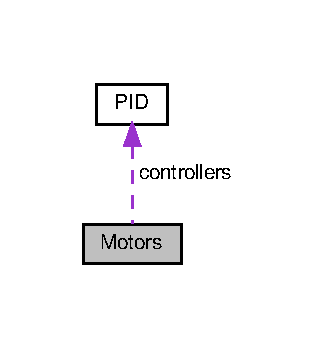
\includegraphics[width=153pt]{structMotors__coll__graph}
\end{center}
\end{figure}
\subsection*{Public Member Functions}
\begin{DoxyCompactItemize}
\item 
\mbox{\Hypertarget{structMotors_ac6532a754e5f1743ee4975b6722b4054}\label{structMotors_ac6532a754e5f1743ee4975b6722b4054}} 
void \hyperlink{structMotors_ac6532a754e5f1743ee4975b6722b4054}{power} ()
\begin{DoxyCompactList}\small\item\em Set power to the motors using the current thrust vector. \end{DoxyCompactList}\item 
\mbox{\Hypertarget{structMotors_a179c6a24115935994a13493f74f56df8}\label{structMotors_a179c6a24115935994a13493f74f56df8}} 
void \hyperlink{structMotors_a179c6a24115935994a13493f74f56df8}{pause} ()
\begin{DoxyCompactList}\small\item\em Pause power to the motors. \end{DoxyCompactList}\item 
uint32\+\_\+t \hyperlink{structMotors_a0d3909ec9fadbb3028368e7340a2e707}{run} (float $\ast$dstate, float $\ast$angles, uint32\+\_\+t t)
\begin{DoxyCompactList}\small\item\em Run the motors for one iteration towards the desired state. \end{DoxyCompactList}\end{DoxyCompactItemize}
\subsection*{Data Fields}
\begin{DoxyCompactItemize}
\item 
\hyperlink{structPID}{P\+ID} \hyperlink{structMotors_a7cbe4b9467412e4882ff318b9375017e}{controllers} \mbox{[}\hyperlink{config_8h_ab5c558d88abd9517fb657be4889ee1bc}{D\+OF}\mbox{]}
\item 
float \hyperlink{structMotors_ac8d20987287ffda85eed109c3bf80a12}{thrust} \mbox{[}\hyperlink{config_8h_ae84658f12c2f1b44f59af36678cf3dcc}{N\+U\+M\+\_\+\+M\+O\+T\+O\+RS}\mbox{]}
\item 
int \hyperlink{structMotors_a84b2ea1a929743410df7ead8212b767a}{buttons} \mbox{[}\hyperlink{config_8h_ae84658f12c2f1b44f59af36678cf3dcc}{N\+U\+M\+\_\+\+M\+O\+T\+O\+RS}\mbox{]}
\item 
float \hyperlink{structMotors_a17cb9b1c3fc7749984c4622439901f84}{forces} \mbox{[}\hyperlink{config_8h_ab5c558d88abd9517fb657be4889ee1bc}{D\+OF}\mbox{]}
\item 
float \hyperlink{structMotors_a94c46cb5dab8c60c9fae75cc6b7af629}{pid} \mbox{[}\hyperlink{config_8h_ab5c558d88abd9517fb657be4889ee1bc}{D\+OF}\mbox{]}
\item 
float \hyperlink{structMotors_a46e39ac60edebef57fca46f878e2c0b5}{p}
\end{DoxyCompactItemize}


\subsection{Detailed Description}
Helper class for motors. 

\subsection{Member Function Documentation}
\mbox{\Hypertarget{structMotors_a0d3909ec9fadbb3028368e7340a2e707}\label{structMotors_a0d3909ec9fadbb3028368e7340a2e707}} 
\index{Motors@{Motors}!run@{run}}
\index{run@{run}!Motors@{Motors}}
\subsubsection{\texorpdfstring{run()}{run()}}
{\footnotesize\ttfamily uint32\+\_\+t Motors\+::run (\begin{DoxyParamCaption}\item[{float $\ast$}]{dstate,  }\item[{float $\ast$}]{angles,  }\item[{uint32\+\_\+t}]{t }\end{DoxyParamCaption})}



Run the motors for one iteration towards the desired state. 


\begin{DoxyParams}{Parameters}
{\em dstate} & Difference between desired and current state. \\
\hline
{\em angles} & Current euler angles. \\
\hline
{\em t} & Current time used for time difference calculations. \\
\hline
\end{DoxyParams}
\begin{DoxyReturn}{Returns}
Time after iteration is finished. 
\end{DoxyReturn}


\subsection{Field Documentation}
\mbox{\Hypertarget{structMotors_a84b2ea1a929743410df7ead8212b767a}\label{structMotors_a84b2ea1a929743410df7ead8212b767a}} 
\index{Motors@{Motors}!buttons@{buttons}}
\index{buttons@{buttons}!Motors@{Motors}}
\subsubsection{\texorpdfstring{buttons}{buttons}}
{\footnotesize\ttfamily int Motors\+::buttons\mbox{[}\hyperlink{config_8h_ae84658f12c2f1b44f59af36678cf3dcc}{N\+U\+M\+\_\+\+M\+O\+T\+O\+RS}\mbox{]}}

Holds pressed values for remote control. \mbox{\Hypertarget{structMotors_a7cbe4b9467412e4882ff318b9375017e}\label{structMotors_a7cbe4b9467412e4882ff318b9375017e}} 
\index{Motors@{Motors}!controllers@{controllers}}
\index{controllers@{controllers}!Motors@{Motors}}
\subsubsection{\texorpdfstring{controllers}{controllers}}
{\footnotesize\ttfamily \hyperlink{structPID}{P\+ID} Motors\+::controllers\mbox{[}\hyperlink{config_8h_ab5c558d88abd9517fb657be4889ee1bc}{D\+OF}\mbox{]}}

\hyperlink{structPID}{P\+ID} controllers for each degree of freedom. \mbox{\Hypertarget{structMotors_a17cb9b1c3fc7749984c4622439901f84}\label{structMotors_a17cb9b1c3fc7749984c4622439901f84}} 
\index{Motors@{Motors}!forces@{forces}}
\index{forces@{forces}!Motors@{Motors}}
\subsubsection{\texorpdfstring{forces}{forces}}
{\footnotesize\ttfamily float Motors\+::forces\mbox{[}\hyperlink{config_8h_ab5c558d88abd9517fb657be4889ee1bc}{D\+OF}\mbox{]}}

Theoretical forces for each degree of freedom. \mbox{\Hypertarget{structMotors_a46e39ac60edebef57fca46f878e2c0b5}\label{structMotors_a46e39ac60edebef57fca46f878e2c0b5}} 
\index{Motors@{Motors}!p@{p}}
\index{p@{p}!Motors@{Motors}}
\subsubsection{\texorpdfstring{p}{p}}
{\footnotesize\ttfamily float Motors\+::p}

Current submarine power. \mbox{\Hypertarget{structMotors_a94c46cb5dab8c60c9fae75cc6b7af629}\label{structMotors_a94c46cb5dab8c60c9fae75cc6b7af629}} 
\index{Motors@{Motors}!pid@{pid}}
\index{pid@{pid}!Motors@{Motors}}
\subsubsection{\texorpdfstring{pid}{pid}}
{\footnotesize\ttfamily float Motors\+::pid\mbox{[}\hyperlink{config_8h_ab5c558d88abd9517fb657be4889ee1bc}{D\+OF}\mbox{]}}

Computed \hyperlink{structPID}{P\+ID} values from each controller. \mbox{\Hypertarget{structMotors_ac8d20987287ffda85eed109c3bf80a12}\label{structMotors_ac8d20987287ffda85eed109c3bf80a12}} 
\index{Motors@{Motors}!thrust@{thrust}}
\index{thrust@{thrust}!Motors@{Motors}}
\subsubsection{\texorpdfstring{thrust}{thrust}}
{\footnotesize\ttfamily float Motors\+::thrust\mbox{[}\hyperlink{config_8h_ae84658f12c2f1b44f59af36678cf3dcc}{N\+U\+M\+\_\+\+M\+O\+T\+O\+RS}\mbox{]}}

Current thrust values for each of the motors. 

The documentation for this struct was generated from the following files\+:\begin{DoxyCompactItemize}
\item 
include/\hyperlink{motor_8hpp}{motor.\+hpp}\item 
src/motor.\+cpp\end{DoxyCompactItemize}

\hypertarget{structparser__var__t}{}\section{parser\+\_\+var\+\_\+t Struct Reference}
\label{structparser__var__t}\index{parser\+\_\+var\+\_\+t@{parser\+\_\+var\+\_\+t}}
\subsection*{Data Fields}
\begin{DoxyCompactItemize}
\item 
\mbox{\Hypertarget{structparser__var__t_aaa58b57d8eae02a80455ab75fb540423}\label{structparser__var__t_aaa58b57d8eae02a80455ab75fb540423}} 
rx\+\_\+state\+\_\+t {\bfseries rx\+\_\+state}
\item 
\mbox{\Hypertarget{structparser__var__t_a54ea3ec01f8166255d8caf8365ab70d8}\label{structparser__var__t_a54ea3ec01f8166255d8caf8365ab70d8}} 
uint16\+\_\+t {\bfseries datagram\+\_\+bytecount}
\item 
\mbox{\Hypertarget{structparser__var__t_a883bea3ba932d1eff0b0d7b1950c3dee}\label{structparser__var__t_a883bea3ba932d1eff0b0d7b1950c3dee}} 
uint8\+\_\+t {\bfseries num\+\_\+data\+\_\+types}
\item 
\mbox{\Hypertarget{structparser__var__t_aa90ac5e2aeae2c80d72ad35cdb06849e}\label{structparser__var__t_aa90ac5e2aeae2c80d72ad35cdb06849e}} 
uint16\+\_\+t {\bfseries offsets} \mbox{[}4\mbox{]}
\item 
\mbox{\Hypertarget{structparser__var__t_ac85fdb6c123d6a3d8cfc12387b73d28b}\label{structparser__var__t_ac85fdb6c123d6a3d8cfc12387b73d28b}} 
uint8\+\_\+t {\bfseries offset\+\_\+loop\+\_\+idx}
\item 
\mbox{\Hypertarget{structparser__var__t_a1932f31a613c5b65f9be6ad970d9fcbc}\label{structparser__var__t_a1932f31a613c5b65f9be6ad970d9fcbc}} 
uint16\+\_\+t {\bfseries rx\+\_\+wait\+\_\+bytecount}
\item 
\mbox{\Hypertarget{structparser__var__t_a79baf5586f5cc330803eb6d2bd2c6b25}\label{structparser__var__t_a79baf5586f5cc330803eb6d2bd2c6b25}} 
uint8\+\_\+t {\bfseries offset\+\_\+wait\+\_\+idx}
\item 
\mbox{\Hypertarget{structparser__var__t_a135aa2aef2d738778acdebf0aff931b1}\label{structparser__var__t_a135aa2aef2d738778acdebf0aff931b1}} 
uint16\+\_\+t {\bfseries frame\+\_\+id}
\item 
\mbox{\Hypertarget{structparser__var__t_a1f4a0b81c336ec7bf8aa3d0bae0dd191}\label{structparser__var__t_a1f4a0b81c336ec7bf8aa3d0bae0dd191}} 
uint8\+\_\+t {\bfseries velocity\+\_\+sb\+\_\+byte\+\_\+idx}
\item 
\mbox{\Hypertarget{structparser__var__t_ad84bccea45c09dd8252328dbc6b7e649}\label{structparser__var__t_ad84bccea45c09dd8252328dbc6b7e649}} 
uint8\+\_\+t {\bfseries velocity\+\_\+fw\+\_\+byte\+\_\+idx}
\item 
\mbox{\Hypertarget{structparser__var__t_a92e32f148ac0f8aa7f77bdc90513ba13}\label{structparser__var__t_a92e32f148ac0f8aa7f77bdc90513ba13}} 
uint8\+\_\+t {\bfseries velocity\+\_\+up\+\_\+byte\+\_\+idx}
\item 
\mbox{\Hypertarget{structparser__var__t_ae5b70f178be99e8cde20be5ee53b5310}\label{structparser__var__t_ae5b70f178be99e8cde20be5ee53b5310}} 
uint8\+\_\+t {\bfseries range\+\_\+byte\+\_\+idx}
\end{DoxyCompactItemize}


The documentation for this struct was generated from the following file\+:\begin{DoxyCompactItemize}
\item 
src/dvl/dvl.\+cpp\end{DoxyCompactItemize}

\hypertarget{structPID}{}\section{P\+ID Struct Reference}
\label{structPID}\index{P\+ID@{P\+ID}}
\subsection*{Public Member Functions}
\begin{DoxyCompactItemize}
\item 
\mbox{\Hypertarget{structPID_ac5b3e2a5ad35e07517f40b8164821f8e}\label{structPID_ac5b3e2a5ad35e07517f40b8164821f8e}} 
{\bfseries P\+ID} (float a, float b, float c)
\item 
\mbox{\Hypertarget{structPID_a43370ace90e60c06253f9322101e3517}\label{structPID_a43370ace90e60c06253f9322101e3517}} 
float {\bfseries init} (float a, float b, float c)
\item 
\mbox{\Hypertarget{structPID_a7d7903c58db1a8b6c63a6f40672d3765}\label{structPID_a7d7903c58db1a8b6c63a6f40672d3765}} 
float {\bfseries calculate} (float error, float dt, float min)
\end{DoxyCompactItemize}
\subsection*{Data Fields}
\begin{DoxyCompactItemize}
\item 
\mbox{\Hypertarget{structPID_a9bff6d497fdd262f6f0f74a76604d22a}\label{structPID_a9bff6d497fdd262f6f0f74a76604d22a}} 
float {\bfseries kp}
\item 
\mbox{\Hypertarget{structPID_af2b185d6025a735e294c3ca698562648}\label{structPID_af2b185d6025a735e294c3ca698562648}} 
float {\bfseries ki}
\item 
\mbox{\Hypertarget{structPID_ac8f8dd4ddd347ff859db4e1dc3af90d5}\label{structPID_ac8f8dd4ddd347ff859db4e1dc3af90d5}} 
float {\bfseries kd}
\item 
\mbox{\Hypertarget{structPID_ab1935e94bf22e1c6f8565a0677ab0871}\label{structPID_ab1935e94bf22e1c6f8565a0677ab0871}} 
float {\bfseries prev}
\item 
\mbox{\Hypertarget{structPID_a04f280906a9f186e64100b3a58775a71}\label{structPID_a04f280906a9f186e64100b3a58775a71}} 
float {\bfseries sum}
\end{DoxyCompactItemize}


The documentation for this struct was generated from the following files\+:\begin{DoxyCompactItemize}
\item 
include/\hyperlink{pid_8hpp}{pid.\+hpp}\item 
src/pid.\+cpp\end{DoxyCompactItemize}

\chapter{File Documentation}
\hypertarget{ahrs_8h}{}\section{include/ahrs/ahrs.h File Reference}
\label{ahrs_8h}\index{include/ahrs/ahrs.\+h@{include/ahrs/ahrs.\+h}}


Interface function definitions for the A\+H\+RS.  


{\ttfamily \#include $<$stdbool.\+h$>$}\newline
Include dependency graph for ahrs.\+h\+:\nopagebreak
\begin{figure}[H]
\begin{center}
\leavevmode
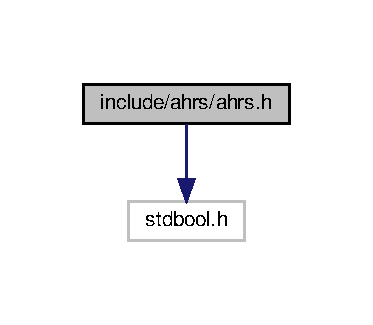
\includegraphics[width=179pt]{ahrs_8h__incl}
\end{center}
\end{figure}
\subsection*{Enumerations}
\begin{DoxyCompactItemize}
\item 
\mbox{\Hypertarget{ahrs_8h_a726ca809ffd3d67ab4b8476646f26635}\label{ahrs_8h_a726ca809ffd3d67ab4b8476646f26635}} 
enum \{ {\bfseries C\+O\+M\+P\+O\+N\+E\+N\+T\+\_\+\+M\+IN}, 
{\bfseries C\+O\+M\+P\+O\+N\+E\+N\+T\+\_\+\+M\+AX}
 \}
\item 
\mbox{\Hypertarget{ahrs_8h_a32d66f8d6f6a878b79f6a18c18fb85cf}\label{ahrs_8h_a32d66f8d6f6a878b79f6a18c18fb85cf}} 
enum {\bfseries att\+\_\+axis} \{ {\bfseries Y\+AW}, 
{\bfseries P\+I\+T\+CH}, 
{\bfseries R\+O\+LL}, 
{\bfseries N\+U\+M\+\_\+\+A\+T\+T\+\_\+\+A\+X\+ES}
 \}
\item 
\mbox{\Hypertarget{ahrs_8h_a98e4c2ebd3776f2226e168117904d6c1}\label{ahrs_8h_a98e4c2ebd3776f2226e168117904d6c1}} 
enum {\bfseries accel\+\_\+axis} \{ {\bfseries S\+W\+AY}, 
{\bfseries H\+E\+A\+VE}, 
{\bfseries S\+U\+R\+GE}, 
{\bfseries N\+U\+M\+\_\+\+A\+C\+C\+E\+L\+\_\+\+A\+X\+ES}
 \}
\end{DoxyCompactItemize}
\subsection*{Functions}
\begin{DoxyCompactItemize}
\item 
int \hyperlink{ahrs_8h_a653d935b0864f7e1ee7aa4dfbb522fcc}{ahrs\+\_\+cont\+\_\+start} ()
\begin{DoxyCompactList}\small\item\em Tells A\+H\+RS to start sending data in continous mode. \end{DoxyCompactList}\item 
float \hyperlink{ahrs_8h_a8432ad8e6e8fcc865fbb5d4e374b7c59}{ahrs\+\_\+att} (enum att\+\_\+axis dir)
\begin{DoxyCompactList}\small\item\em Tells A\+H\+RS to return angle for a certain direction. \end{DoxyCompactList}\item 
float \hyperlink{ahrs_8h_a49574e1c0ff13ef5edd5ea8d4d3d2914}{ahrs\+\_\+accel} (enum accel\+\_\+axis dir)
\begin{DoxyCompactList}\small\item\em Tells A\+H\+RS to return acceleration for certain direction. \end{DoxyCompactList}\item 
uint\+\_\+fast8\+\_\+t \hyperlink{ahrs_8h_aabcd9bcc5487394de174cb4b78f01d25}{ahrs\+\_\+headingstatus} ()
\begin{DoxyCompactList}\small\item\em Tells A\+H\+RS to return accuracy of current data. \end{DoxyCompactList}\item 
bool \hyperlink{ahrs_8h_a13682875d497e50e1b7bf5e5d173e154}{ahrs\+\_\+att\+\_\+update} ()
\begin{DoxyCompactList}\small\item\em Updates A\+H\+RS data. \end{DoxyCompactList}\item 
int \hyperlink{ahrs_8h_a9298af19f8651e14c0f43505c2196876}{ahrs\+\_\+att\+\_\+recv} ()
\begin{DoxyCompactList}\small\item\em Determines whether A\+H\+RS is returning data. \end{DoxyCompactList}\item 
void \hyperlink{ahrs_8h_a76fe8dc1638d7c89f7e14bc86238283c}{ahrs\+\_\+parse\+\_\+att\+\_\+reset} ()
\begin{DoxyCompactList}\small\item\em Discards incomplete A\+H\+RS data. \end{DoxyCompactList}\item 
\mbox{\Hypertarget{ahrs_8h_aa55ad38ec0330c9981d4d25742d1bb65}\label{ahrs_8h_aa55ad38ec0330c9981d4d25742d1bb65}} 
int {\bfseries ahrs\+\_\+set\+\_\+datacomp} ()
\end{DoxyCompactItemize}
\subsection*{Variables}
\begin{DoxyCompactItemize}
\item 
\mbox{\Hypertarget{ahrs_8h_a4f242cea3e7c041553bf2648729d6598}\label{ahrs_8h_a4f242cea3e7c041553bf2648729d6598}} 
float const {\bfseries ahrs\+\_\+range} \mbox{[}N\+U\+M\+\_\+\+A\+T\+T\+\_\+\+A\+X\+ES\mbox{]}\mbox{[}2\mbox{]}
\end{DoxyCompactItemize}


\subsection{Detailed Description}
Interface function definitions for the A\+H\+RS. 

\begin{DoxyAuthor}{Author}
Seth Girvan (Lord) 
\end{DoxyAuthor}


\subsection{Function Documentation}
\mbox{\Hypertarget{ahrs_8h_a49574e1c0ff13ef5edd5ea8d4d3d2914}\label{ahrs_8h_a49574e1c0ff13ef5edd5ea8d4d3d2914}} 
\index{ahrs.\+h@{ahrs.\+h}!ahrs\+\_\+accel@{ahrs\+\_\+accel}}
\index{ahrs\+\_\+accel@{ahrs\+\_\+accel}!ahrs.\+h@{ahrs.\+h}}
\subsubsection{\texorpdfstring{ahrs\+\_\+accel()}{ahrs\_accel()}}
{\footnotesize\ttfamily float ahrs\+\_\+accel (\begin{DoxyParamCaption}\item[{enum accel\+\_\+axis}]{dir }\end{DoxyParamCaption})}



Tells A\+H\+RS to return acceleration for certain direction. 

The coordinates are left-\/handed with positive heave up, positive sway left, and positive surge back.


\begin{DoxyParams}{Parameters}
{\em dir} & The wanted direction. \\
\hline
\end{DoxyParams}
\begin{DoxyReturn}{Returns}
The accelerometer value in G received from the ahrs for the dir. 
\end{DoxyReturn}
\mbox{\Hypertarget{ahrs_8h_a8432ad8e6e8fcc865fbb5d4e374b7c59}\label{ahrs_8h_a8432ad8e6e8fcc865fbb5d4e374b7c59}} 
\index{ahrs.\+h@{ahrs.\+h}!ahrs\+\_\+att@{ahrs\+\_\+att}}
\index{ahrs\+\_\+att@{ahrs\+\_\+att}!ahrs.\+h@{ahrs.\+h}}
\subsubsection{\texorpdfstring{ahrs\+\_\+att()}{ahrs\_att()}}
{\footnotesize\ttfamily float ahrs\+\_\+att (\begin{DoxyParamCaption}\item[{enum att\+\_\+axis}]{dir }\end{DoxyParamCaption})}



Tells A\+H\+RS to return angle for a certain direction. 

If the ahrs is in degrees mode the values will range per ahrs\+\_\+range\mbox{[}dir\mbox{]}.

The values returned will not changed until \hyperlink{ahrs_8h_a13682875d497e50e1b7bf5e5d173e154}{ahrs\+\_\+att\+\_\+update()} is called and it returns true.


\begin{DoxyParams}{Parameters}
{\em dir} & The wanted direction. \\
\hline
\end{DoxyParams}
\begin{DoxyReturn}{Returns}
The value received from the ahrs for the passed direction. 
\end{DoxyReturn}
\mbox{\Hypertarget{ahrs_8h_a9298af19f8651e14c0f43505c2196876}\label{ahrs_8h_a9298af19f8651e14c0f43505c2196876}} 
\index{ahrs.\+h@{ahrs.\+h}!ahrs\+\_\+att\+\_\+recv@{ahrs\+\_\+att\+\_\+recv}}
\index{ahrs\+\_\+att\+\_\+recv@{ahrs\+\_\+att\+\_\+recv}!ahrs.\+h@{ahrs.\+h}}
\subsubsection{\texorpdfstring{ahrs\+\_\+att\+\_\+recv()}{ahrs\_att\_recv()}}
{\footnotesize\ttfamily int ahrs\+\_\+att\+\_\+recv (\begin{DoxyParamCaption}{ }\end{DoxyParamCaption})}



Determines whether A\+H\+RS is returning data. 

\begin{DoxyReturn}{Returns}
True if at least one valid data set has been completely read from the ahrs. 
\end{DoxyReturn}
\mbox{\Hypertarget{ahrs_8h_a13682875d497e50e1b7bf5e5d173e154}\label{ahrs_8h_a13682875d497e50e1b7bf5e5d173e154}} 
\index{ahrs.\+h@{ahrs.\+h}!ahrs\+\_\+att\+\_\+update@{ahrs\+\_\+att\+\_\+update}}
\index{ahrs\+\_\+att\+\_\+update@{ahrs\+\_\+att\+\_\+update}!ahrs.\+h@{ahrs.\+h}}
\subsubsection{\texorpdfstring{ahrs\+\_\+att\+\_\+update()}{ahrs\_att\_update()}}
{\footnotesize\ttfamily bool ahrs\+\_\+att\+\_\+update (\begin{DoxyParamCaption}{ }\end{DoxyParamCaption})}



Updates A\+H\+RS data. 

Updates the values returned by ahrs\+\_\+att to the newest complete set of data that has been received from the ahrs before some point in time within this function\textquotesingle{}s lifetime.

Should only be called between complete \char`\"{}uses\char`\"{} of the attitude data to avoid using disparate data together (ie between runs of a \hyperlink{structPID}{P\+ID} routine).

\begin{DoxyReturn}{Returns}
True when there has been a new complete set of data received from the ahrs since the last time \hyperlink{ahrs_8h_a13682875d497e50e1b7bf5e5d173e154}{ahrs\+\_\+att\+\_\+update()} has been called. 
\end{DoxyReturn}
\mbox{\Hypertarget{ahrs_8h_a653d935b0864f7e1ee7aa4dfbb522fcc}\label{ahrs_8h_a653d935b0864f7e1ee7aa4dfbb522fcc}} 
\index{ahrs.\+h@{ahrs.\+h}!ahrs\+\_\+cont\+\_\+start@{ahrs\+\_\+cont\+\_\+start}}
\index{ahrs\+\_\+cont\+\_\+start@{ahrs\+\_\+cont\+\_\+start}!ahrs.\+h@{ahrs.\+h}}
\subsubsection{\texorpdfstring{ahrs\+\_\+cont\+\_\+start()}{ahrs\_cont\_start()}}
{\footnotesize\ttfamily int ahrs\+\_\+cont\+\_\+start (\begin{DoxyParamCaption}{ }\end{DoxyParamCaption})}



Tells A\+H\+RS to start sending data in continous mode. 

Make sure the desired data components are set first, such as with ahrs\+\_\+set\+\_\+datacomp().

\begin{DoxyReturn}{Returns}
0 on success 
\end{DoxyReturn}
\mbox{\Hypertarget{ahrs_8h_aabcd9bcc5487394de174cb4b78f01d25}\label{ahrs_8h_aabcd9bcc5487394de174cb4b78f01d25}} 
\index{ahrs.\+h@{ahrs.\+h}!ahrs\+\_\+headingstatus@{ahrs\+\_\+headingstatus}}
\index{ahrs\+\_\+headingstatus@{ahrs\+\_\+headingstatus}!ahrs.\+h@{ahrs.\+h}}
\subsubsection{\texorpdfstring{ahrs\+\_\+headingstatus()}{ahrs\_headingstatus()}}
{\footnotesize\ttfamily uint\+\_\+fast8\+\_\+t ahrs\+\_\+headingstatus (\begin{DoxyParamCaption}{ }\end{DoxyParamCaption})}



Tells A\+H\+RS to return accuracy of current data. 

Values\+: 1\+: uncertainty less than 2 degrees 2\+: uncertainty between 2 and 10 degres 3\+: uncertainty greater than 10 degrees However, it may give other values (I have known it to give the value 0).

\begin{DoxyReturn}{Returns}
The k\+Heading\+Status component from the ahrs associated with the current attitude data. 
\end{DoxyReturn}
\mbox{\Hypertarget{ahrs_8h_a76fe8dc1638d7c89f7e14bc86238283c}\label{ahrs_8h_a76fe8dc1638d7c89f7e14bc86238283c}} 
\index{ahrs.\+h@{ahrs.\+h}!ahrs\+\_\+parse\+\_\+att\+\_\+reset@{ahrs\+\_\+parse\+\_\+att\+\_\+reset}}
\index{ahrs\+\_\+parse\+\_\+att\+\_\+reset@{ahrs\+\_\+parse\+\_\+att\+\_\+reset}!ahrs.\+h@{ahrs.\+h}}
\subsubsection{\texorpdfstring{ahrs\+\_\+parse\+\_\+att\+\_\+reset()}{ahrs\_parse\_att\_reset()}}
{\footnotesize\ttfamily void ahrs\+\_\+parse\+\_\+att\+\_\+reset (\begin{DoxyParamCaption}{ }\end{DoxyParamCaption})}



Discards incomplete A\+H\+RS data. 

Causes any data from a current incomplete datagram to be discarded. The next received byte will be treated as potentially the start of a datagram.

Can be used due for, eg, a serial timeout for intra-\/datagram data. 
\hypertarget{crc__xmodem_8h}{}\section{include/ahrs/crc\+\_\+xmodem.h File Reference}
\label{crc__xmodem_8h}\index{include/ahrs/crc\+\_\+xmodem.\+h@{include/ahrs/crc\+\_\+xmodem.\+h}}


Helper macros for C\+R\+C-\/\+X\+M\+O\+D\+EM updating.  


{\ttfamily \#include \char`\"{}crc\+\_\+xmodem\+\_\+generic.\+h\char`\"{}}\newline
Include dependency graph for crc\+\_\+xmodem.\+h\+:
\nopagebreak
\begin{figure}[H]
\begin{center}
\leavevmode
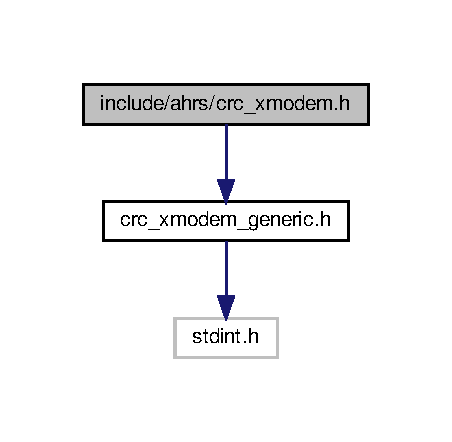
\includegraphics[width=217pt]{crc__xmodem_8h__incl}
\end{center}
\end{figure}
\subsection*{Macros}
\begin{DoxyCompactItemize}
\item 
\mbox{\Hypertarget{crc__xmodem_8h_abb06933ed9907921f240b9d301855d25}\label{crc__xmodem_8h_abb06933ed9907921f240b9d301855d25}} 
\#define {\bfseries C\+R\+C\+\_\+\+X\+M\+O\+D\+E\+M\+\_\+\+I\+N\+I\+T\+\_\+\+V\+AL}~0x0000U
\item 
\mbox{\Hypertarget{crc__xmodem_8h_a12fd495ff0805ef2335ae91a5de4a94e}\label{crc__xmodem_8h_a12fd495ff0805ef2335ae91a5de4a94e}} 
\#define {\bfseries crc\+\_\+xmodem\+\_\+update}(a,  b)~\hyperlink{crc__xmodem__generic_8h_a618a4e92162fc58fd2f3b8ba0b452e67}{generic\+\_\+crc\+\_\+xmodem\+\_\+update}(a, b)
\end{DoxyCompactItemize}


\subsection{Detailed Description}
Helper macros for C\+R\+C-\/\+X\+M\+O\+D\+EM updating. 

\begin{DoxyAuthor}{Author}
Seth Girvan (Lord) 
\end{DoxyAuthor}

\hypertarget{crc__xmodem__generic_8h}{}\section{include/ahrs/crc\+\_\+xmodem\+\_\+generic.h File Reference}
\label{crc__xmodem__generic_8h}\index{include/ahrs/crc\+\_\+xmodem\+\_\+generic.\+h@{include/ahrs/crc\+\_\+xmodem\+\_\+generic.\+h}}


C\+RC update functions for testing.  


{\ttfamily \#include $<$stdint.\+h$>$}\newline
Include dependency graph for crc\+\_\+xmodem\+\_\+generic.\+h\+:\nopagebreak
\begin{figure}[H]
\begin{center}
\leavevmode
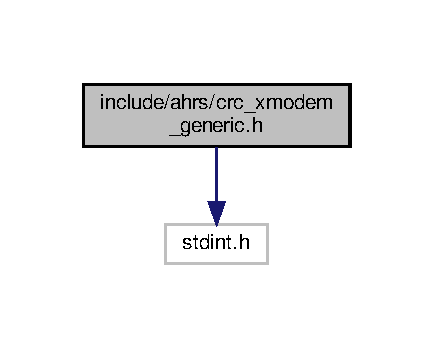
\includegraphics[width=208pt]{crc__xmodem__generic_8h__incl}
\end{center}
\end{figure}
This graph shows which files directly or indirectly include this file\+:\nopagebreak
\begin{figure}[H]
\begin{center}
\leavevmode
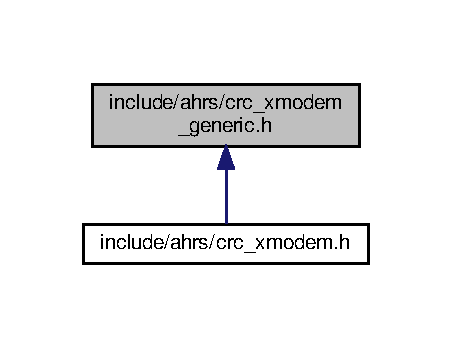
\includegraphics[width=217pt]{crc__xmodem__generic_8h__dep__incl}
\end{center}
\end{figure}
\subsection*{Functions}
\begin{DoxyCompactItemize}
\item 
uint16\+\_\+t \hyperlink{crc__xmodem__generic_8h_a618a4e92162fc58fd2f3b8ba0b452e67}{generic\+\_\+crc\+\_\+xmodem\+\_\+update} (uint16\+\_\+t crc, uint8\+\_\+t data)
\begin{DoxyCompactList}\small\item\em Update a C\+RC with 8 bits of additional data. \end{DoxyCompactList}\end{DoxyCompactItemize}


\subsection{Detailed Description}
C\+RC update functions for testing. 

\begin{DoxyAuthor}{Author}
Seth Girvan (Lord) 
\end{DoxyAuthor}


\subsection{Function Documentation}
\mbox{\Hypertarget{crc__xmodem__generic_8h_a618a4e92162fc58fd2f3b8ba0b452e67}\label{crc__xmodem__generic_8h_a618a4e92162fc58fd2f3b8ba0b452e67}} 
\index{crc\+\_\+xmodem\+\_\+generic.\+h@{crc\+\_\+xmodem\+\_\+generic.\+h}!generic\+\_\+crc\+\_\+xmodem\+\_\+update@{generic\+\_\+crc\+\_\+xmodem\+\_\+update}}
\index{generic\+\_\+crc\+\_\+xmodem\+\_\+update@{generic\+\_\+crc\+\_\+xmodem\+\_\+update}!crc\+\_\+xmodem\+\_\+generic.\+h@{crc\+\_\+xmodem\+\_\+generic.\+h}}
\subsubsection{\texorpdfstring{generic\+\_\+crc\+\_\+xmodem\+\_\+update()}{generic\_crc\_xmodem\_update()}}
{\footnotesize\ttfamily uint16\+\_\+t generic\+\_\+crc\+\_\+xmodem\+\_\+update (\begin{DoxyParamCaption}\item[{uint16\+\_\+t}]{crc,  }\item[{uint8\+\_\+t}]{data }\end{DoxyParamCaption})}



Update a C\+RC with 8 bits of additional data. 

This is unoptimized and meant to be used for testing on computer. On avr, one should use the optimized \+\_\+crc\+\_\+xmodem\+\_\+update() in util/crc16.\+h

\begin{DoxyReturn}{Returns}
New C\+RC. 
\end{DoxyReturn}

\hypertarget{io__ahrs_8h}{}\section{include/ahrs/io\+\_\+ahrs.h File Reference}
\label{io__ahrs_8h}\index{include/ahrs/io\+\_\+ahrs.\+h@{include/ahrs/io\+\_\+ahrs.\+h}}


Low-\/level communication functions for A\+H\+RS.  


{\ttfamily \#include $<$stdio.\+h$>$}\newline
{\ttfamily \#include $<$stdbool.\+h$>$}\newline
Include dependency graph for io\+\_\+ahrs.\+h\+:
\nopagebreak
\begin{figure}[H]
\begin{center}
\leavevmode
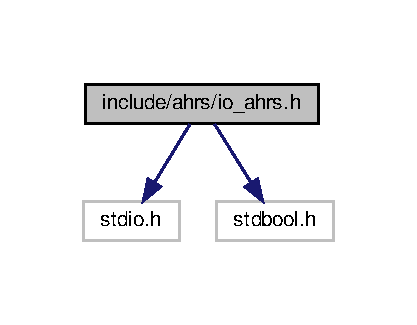
\includegraphics[width=200pt]{io__ahrs_8h__incl}
\end{center}
\end{figure}
\subsection*{Functions}
\begin{DoxyCompactItemize}
\item 
void \hyperlink{io__ahrs_8h_a312fc51f6c9726e41cfbc780cfcfecdc}{io\+\_\+ahrs\+\_\+init} (char const $\ast$path)
\begin{DoxyCompactList}\small\item\em Prepare A\+H\+RS to receive data. \end{DoxyCompactList}\item 
void \hyperlink{io__ahrs_8h_a9db69393e769bcdd5ddc9ec5f125d11d}{io\+\_\+ahrs\+\_\+clean} ()
\begin{DoxyCompactList}\small\item\em Disable A\+H\+RS transmit and receive. \end{DoxyCompactList}\item 
int \hyperlink{io__ahrs_8h_afa79bf757710a1cad094f1e15eb634b7}{io\+\_\+ahrs\+\_\+recv\+\_\+start} (int($\ast$handler)())
\begin{DoxyCompactList}\small\item\em Tells A\+H\+RS to start receiving attitude data. \end{DoxyCompactList}\item 
void \hyperlink{io__ahrs_8h_a2ee2459ddd2dca694bef3e6fb9b1cd54}{io\+\_\+ahrs\+\_\+recv\+\_\+stop} ()
\begin{DoxyCompactList}\small\item\em Tells A\+H\+RS to start receiving attitude data. \end{DoxyCompactList}\item 
bool \hyperlink{io__ahrs_8h_a7b33a09e7c9290bcdeebf2602a54ee3d}{io\+\_\+ahrs\+\_\+tripbuf\+\_\+update} ()
\item 
void \hyperlink{io__ahrs_8h_ac133fdc94162c623c5325f907ade9e4a}{io\+\_\+ahrs\+\_\+tripbuf\+\_\+offer} ()
\item 
unsigned char \hyperlink{io__ahrs_8h_a7e158c735ff3b4a8b84cd5bd552c4954}{io\+\_\+ahrs\+\_\+tripbuf\+\_\+read} ()
\item 
unsigned char \hyperlink{io__ahrs_8h_a7690920caf5d41a90442ca049336778c}{io\+\_\+ahrs\+\_\+tripbuf\+\_\+write} ()
\end{DoxyCompactItemize}
\subsection*{Variables}
\begin{DoxyCompactItemize}
\item 
F\+I\+LE $\ast$ \hyperlink{io__ahrs_8h_a7c946296e6bffe77d1c08cdcbd4def85}{io\+\_\+ahrs}
\end{DoxyCompactItemize}


\subsection{Detailed Description}
Low-\/level communication functions for A\+H\+RS. 

\begin{DoxyAuthor}{Author}
Seth Girvan (Lord) 
\end{DoxyAuthor}


\subsection{Function Documentation}
\mbox{\Hypertarget{io__ahrs_8h_a9db69393e769bcdd5ddc9ec5f125d11d}\label{io__ahrs_8h_a9db69393e769bcdd5ddc9ec5f125d11d}} 
\index{io\+\_\+ahrs.\+h@{io\+\_\+ahrs.\+h}!io\+\_\+ahrs\+\_\+clean@{io\+\_\+ahrs\+\_\+clean}}
\index{io\+\_\+ahrs\+\_\+clean@{io\+\_\+ahrs\+\_\+clean}!io\+\_\+ahrs.\+h@{io\+\_\+ahrs.\+h}}
\subsubsection{\texorpdfstring{io\+\_\+ahrs\+\_\+clean()}{io\_ahrs\_clean()}}
{\footnotesize\ttfamily void io\+\_\+ahrs\+\_\+clean (\begin{DoxyParamCaption}{ }\end{DoxyParamCaption})}



Disable A\+H\+RS transmit and receive. 

Unimplemented.

\begin{DoxyReturn}{Returns}
Void. 
\end{DoxyReturn}
\mbox{\Hypertarget{io__ahrs_8h_a312fc51f6c9726e41cfbc780cfcfecdc}\label{io__ahrs_8h_a312fc51f6c9726e41cfbc780cfcfecdc}} 
\index{io\+\_\+ahrs.\+h@{io\+\_\+ahrs.\+h}!io\+\_\+ahrs\+\_\+init@{io\+\_\+ahrs\+\_\+init}}
\index{io\+\_\+ahrs\+\_\+init@{io\+\_\+ahrs\+\_\+init}!io\+\_\+ahrs.\+h@{io\+\_\+ahrs.\+h}}
\subsubsection{\texorpdfstring{io\+\_\+ahrs\+\_\+init()}{io\_ahrs\_init()}}
{\footnotesize\ttfamily void io\+\_\+ahrs\+\_\+init (\begin{DoxyParamCaption}\item[{char const $\ast$}]{path }\end{DoxyParamCaption})}



Prepare A\+H\+RS to receive data. 

Assumes uart N\+U\+S\+A\+RT will be used and connected with the ahrs I\+E\+A-\/232 interface via a ttl$<$-\/$>$I\+E\+A-\/232 converter.

Per the T\+R\+AX P\+NI user manual\+: Start Bits\+: 1 Number of Data Bits\+: 8 Stop Bits\+: 1 Parity\+: none Baud\+: B\+A\+UD


\begin{DoxyParams}{Parameters}
{\em path} & Path to A\+H\+RS from main computer, unused at the moment. \\
\hline
\end{DoxyParams}
\begin{DoxyReturn}{Returns}
Void. 
\end{DoxyReturn}
\mbox{\Hypertarget{io__ahrs_8h_afa79bf757710a1cad094f1e15eb634b7}\label{io__ahrs_8h_afa79bf757710a1cad094f1e15eb634b7}} 
\index{io\+\_\+ahrs.\+h@{io\+\_\+ahrs.\+h}!io\+\_\+ahrs\+\_\+recv\+\_\+start@{io\+\_\+ahrs\+\_\+recv\+\_\+start}}
\index{io\+\_\+ahrs\+\_\+recv\+\_\+start@{io\+\_\+ahrs\+\_\+recv\+\_\+start}!io\+\_\+ahrs.\+h@{io\+\_\+ahrs.\+h}}
\subsubsection{\texorpdfstring{io\+\_\+ahrs\+\_\+recv\+\_\+start()}{io\_ahrs\_recv\_start()}}
{\footnotesize\ttfamily int io\+\_\+ahrs\+\_\+recv\+\_\+start (\begin{DoxyParamCaption}\item[{int($\ast$)()}]{handler }\end{DoxyParamCaption})}



Tells A\+H\+RS to start receiving attitude data. 

\begin{DoxyReturn}{Returns}
0 on success 
\end{DoxyReturn}
\mbox{\Hypertarget{io__ahrs_8h_a2ee2459ddd2dca694bef3e6fb9b1cd54}\label{io__ahrs_8h_a2ee2459ddd2dca694bef3e6fb9b1cd54}} 
\index{io\+\_\+ahrs.\+h@{io\+\_\+ahrs.\+h}!io\+\_\+ahrs\+\_\+recv\+\_\+stop@{io\+\_\+ahrs\+\_\+recv\+\_\+stop}}
\index{io\+\_\+ahrs\+\_\+recv\+\_\+stop@{io\+\_\+ahrs\+\_\+recv\+\_\+stop}!io\+\_\+ahrs.\+h@{io\+\_\+ahrs.\+h}}
\subsubsection{\texorpdfstring{io\+\_\+ahrs\+\_\+recv\+\_\+stop()}{io\_ahrs\_recv\_stop()}}
{\footnotesize\ttfamily void io\+\_\+ahrs\+\_\+recv\+\_\+stop (\begin{DoxyParamCaption}{ }\end{DoxyParamCaption})}



Tells A\+H\+RS to start receiving attitude data. 

\begin{DoxyReturn}{Returns}
0 on success 
\end{DoxyReturn}
\mbox{\Hypertarget{io__ahrs_8h_ac133fdc94162c623c5325f907ade9e4a}\label{io__ahrs_8h_ac133fdc94162c623c5325f907ade9e4a}} 
\index{io\+\_\+ahrs.\+h@{io\+\_\+ahrs.\+h}!io\+\_\+ahrs\+\_\+tripbuf\+\_\+offer@{io\+\_\+ahrs\+\_\+tripbuf\+\_\+offer}}
\index{io\+\_\+ahrs\+\_\+tripbuf\+\_\+offer@{io\+\_\+ahrs\+\_\+tripbuf\+\_\+offer}!io\+\_\+ahrs.\+h@{io\+\_\+ahrs.\+h}}
\subsubsection{\texorpdfstring{io\+\_\+ahrs\+\_\+tripbuf\+\_\+offer()}{io\_ahrs\_tripbuf\_offer()}}
{\footnotesize\ttfamily void io\+\_\+ahrs\+\_\+tripbuf\+\_\+offer (\begin{DoxyParamCaption}{ }\end{DoxyParamCaption})}

Makes the current write index available to io\+\_\+ahrs\+\_\+tripbuf\+\_\+update, and changes the value returned by io\+\_\+ahrs\+\_\+tripbuf\+\_\+write.

May interrupt io\+\_\+ahrs\+\_\+tripbuf\+\_\+update, but may not be interrupted by it \mbox{\Hypertarget{io__ahrs_8h_a7e158c735ff3b4a8b84cd5bd552c4954}\label{io__ahrs_8h_a7e158c735ff3b4a8b84cd5bd552c4954}} 
\index{io\+\_\+ahrs.\+h@{io\+\_\+ahrs.\+h}!io\+\_\+ahrs\+\_\+tripbuf\+\_\+read@{io\+\_\+ahrs\+\_\+tripbuf\+\_\+read}}
\index{io\+\_\+ahrs\+\_\+tripbuf\+\_\+read@{io\+\_\+ahrs\+\_\+tripbuf\+\_\+read}!io\+\_\+ahrs.\+h@{io\+\_\+ahrs.\+h}}
\subsubsection{\texorpdfstring{io\+\_\+ahrs\+\_\+tripbuf\+\_\+read()}{io\_ahrs\_tripbuf\_read()}}
{\footnotesize\ttfamily unsigned char io\+\_\+ahrs\+\_\+tripbuf\+\_\+read (\begin{DoxyParamCaption}{ }\end{DoxyParamCaption})}

returns the index of the buffer the data consumer should read from. Only changes if io\+\_\+ahrs\+\_\+tripbuf\+\_\+update is called and returns true. \mbox{\Hypertarget{io__ahrs_8h_a7b33a09e7c9290bcdeebf2602a54ee3d}\label{io__ahrs_8h_a7b33a09e7c9290bcdeebf2602a54ee3d}} 
\index{io\+\_\+ahrs.\+h@{io\+\_\+ahrs.\+h}!io\+\_\+ahrs\+\_\+tripbuf\+\_\+update@{io\+\_\+ahrs\+\_\+tripbuf\+\_\+update}}
\index{io\+\_\+ahrs\+\_\+tripbuf\+\_\+update@{io\+\_\+ahrs\+\_\+tripbuf\+\_\+update}!io\+\_\+ahrs.\+h@{io\+\_\+ahrs.\+h}}
\subsubsection{\texorpdfstring{io\+\_\+ahrs\+\_\+tripbuf\+\_\+update()}{io\_ahrs\_tripbuf\_update()}}
{\footnotesize\ttfamily bool io\+\_\+ahrs\+\_\+tripbuf\+\_\+update (\begin{DoxyParamCaption}{ }\end{DoxyParamCaption})}

Causes io\+\_\+ahrs\+\_\+tripbuf\+\_\+read to return index that was most recently \textquotesingle{}submitted\textquotesingle{} by io\+\_\+ahrs\+\_\+tripbuf\+\_\+offer.

This should only be run between complete \textquotesingle{}uses\textquotesingle{} of the data, to avoid using disparate data.

Unfortunately, since there is no way to have a lock-\/free/interruptable triple buffer implementation on the avr, this has to be platform-\/specific. A lock-\/free ring buffer would not handle cases when the producer is faster than the consumer well.

May be interrupted by io\+\_\+ahrs\+\_\+tripbuf\+\_\+offer, but cannot interrupt it (ie this can be interrupted by handler\+\_\+ahrs\+\_\+recv, but one probably does not want to call it from handler\+\_\+ahrs\+\_\+recv).

returns whether there has been any new data since last call \mbox{\Hypertarget{io__ahrs_8h_a7690920caf5d41a90442ca049336778c}\label{io__ahrs_8h_a7690920caf5d41a90442ca049336778c}} 
\index{io\+\_\+ahrs.\+h@{io\+\_\+ahrs.\+h}!io\+\_\+ahrs\+\_\+tripbuf\+\_\+write@{io\+\_\+ahrs\+\_\+tripbuf\+\_\+write}}
\index{io\+\_\+ahrs\+\_\+tripbuf\+\_\+write@{io\+\_\+ahrs\+\_\+tripbuf\+\_\+write}!io\+\_\+ahrs.\+h@{io\+\_\+ahrs.\+h}}
\subsubsection{\texorpdfstring{io\+\_\+ahrs\+\_\+tripbuf\+\_\+write()}{io\_ahrs\_tripbuf\_write()}}
{\footnotesize\ttfamily unsigned char io\+\_\+ahrs\+\_\+tripbuf\+\_\+write (\begin{DoxyParamCaption}{ }\end{DoxyParamCaption})}

returns the index of the buffer the data producer should write to. Only changes when io\+\_\+ahrs\+\_\+tripbuf\+\_\+offer is called. 

\subsection{Variable Documentation}
\mbox{\Hypertarget{io__ahrs_8h_a7c946296e6bffe77d1c08cdcbd4def85}\label{io__ahrs_8h_a7c946296e6bffe77d1c08cdcbd4def85}} 
\index{io\+\_\+ahrs.\+h@{io\+\_\+ahrs.\+h}!io\+\_\+ahrs@{io\+\_\+ahrs}}
\index{io\+\_\+ahrs@{io\+\_\+ahrs}!io\+\_\+ahrs.\+h@{io\+\_\+ahrs.\+h}}
\subsubsection{\texorpdfstring{io\+\_\+ahrs}{io\_ahrs}}
{\footnotesize\ttfamily F\+I\+LE$\ast$ io\+\_\+ahrs}

io with this is blocking, so one might use normal stdio functions directly on it when they are willing to wait, eg sending initial configuration data, but to be able to handle asynchronous io, one should use io\+\_\+ahrs\+\_\+...\+\_\+start, which allows us to process data on the fly and avoid polling. 
\hypertarget{config_8h}{}\section{include/config.h File Reference}
\label{config_8h}\index{include/config.\+h@{include/config.\+h}}


Configuration options for Nautical.  


This graph shows which files directly or indirectly include this file\+:\nopagebreak
\begin{figure}[H]
\begin{center}
\leavevmode
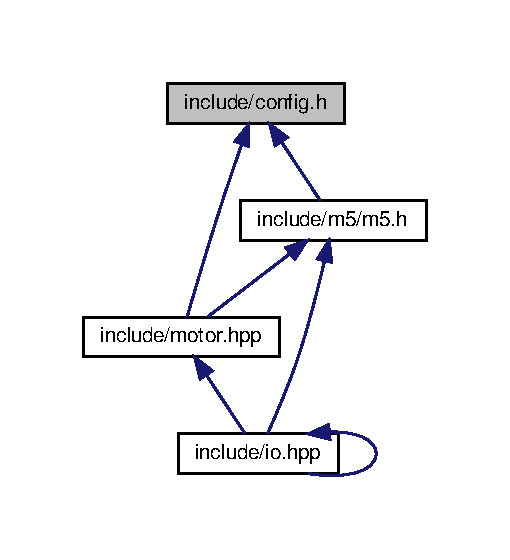
\includegraphics[width=245pt]{config_8h__dep__incl}
\end{center}
\end{figure}
\subsection*{Macros}
\begin{Indent}\textbf{ Conversions.}\par
\begin{DoxyCompactItemize}
\item 
\mbox{\Hypertarget{config_8h_a0a3cc1d5cde549e408f825ddd7f5853d}\label{config_8h_a0a3cc1d5cde549e408f825ddd7f5853d}} 
\#define {\bfseries D2R}~3.\+1415/180.
\item 
\mbox{\Hypertarget{config_8h_a39c663074332446065723e9be9350139}\label{config_8h_a39c663074332446065723e9be9350139}} 
\#define {\bfseries R2D}~180./3.\+1415
\end{DoxyCompactItemize}
\end{Indent}
\subsection*{Variables}
\begin{Indent}\textbf{ Runtime configuration.}\par
\begin{DoxyCompactItemize}
\item 
static const bool \hyperlink{config_8h_a51c905eb4396ee56a3a9c095e3b58bfe}{D\+V\+L\+\_\+\+ON} = false
\item 
static const bool \hyperlink{config_8h_a6d006725140166599b441c1449fc7a3a}{U\+S\+E\+\_\+\+I\+N\+I\+T\+I\+A\+L\+\_\+\+H\+E\+A\+D\+I\+NG} = true
\item 
static const bool \hyperlink{config_8h_a3b5204d43975dfc5858dd3b59eb049bd}{F\+AR} = true
\item 
static const bool \hyperlink{config_8h_a589b4f622d6edccfa6c073a113fa4836}{S\+IM} = false
\end{DoxyCompactItemize}
\end{Indent}
\begin{Indent}\textbf{ Constants for degrees of freedom with North-\/\+East-\/\+Down coordinates.}\par
\begin{DoxyCompactItemize}
\item 
static const int \hyperlink{config_8h_ab5c558d88abd9517fb657be4889ee1bc}{D\+OF} = 6
\item 
static const int \hyperlink{config_8h_a41e6c9e69829719a154249c60cbdf1b2}{B\+O\+D\+Y\+\_\+\+D\+OF} = 3
\item 
static const int \hyperlink{config_8h_a776938745e0d7539a3210a2404305ee6}{G\+Y\+R\+O\+\_\+\+D\+OF} = 6
\item 
static const int \hyperlink{config_8h_a1c83625ec20fd09ecaf0e5b37c75f6f8}{F} = 0
\item 
static const int \hyperlink{config_8h_a0f4b0111b93bf2933b351bba78cc9f79}{H} = 1
\item 
static const int \hyperlink{config_8h_ac5dc2e25ee3e4af146d8ccdb65cf43da}{V} = 2
\item 
static const int \hyperlink{config_8h_a4245f3c5e8eb90ade09427f989b098ec}{Y} = 3
\item 
static const int \hyperlink{config_8h_aabaa1bd1eed76e739bbc16c7e4e72549}{P} = 4
\item 
static const int \hyperlink{config_8h_a554e63228b946db0d44c4f398b18e212}{R} = 5
\end{DoxyCompactItemize}
\end{Indent}
\begin{Indent}\textbf{ Motor orientation configuration.}\par
\begin{DoxyCompactItemize}
\item 
static const float \hyperlink{config_8h_a8925b73125e9fe0a48808f4e2a3f8561}{O\+R\+I\+E\+N\+T\+A\+T\+I\+ON} \mbox{[}8\mbox{]}\mbox{[}6\mbox{]}
\end{DoxyCompactItemize}
\end{Indent}
\begin{Indent}\textbf{ P\+ID gains configuration.}\par
\begin{DoxyCompactItemize}
\item 
static const float \hyperlink{config_8h_a15c324540eac139d826a36cacf0c7e2b}{G\+A\+I\+NS} \mbox{[}6\mbox{]}\mbox{[}3\mbox{]}
\end{DoxyCompactItemize}
\end{Indent}
\subsection*{Motor ID configuration.}
\begin{DoxyCompactItemize}
\item 
enum \hyperlink{config_8h_a2ee7466b8ebcae32e1e733f8067a6f9a}{thruster} \{ \newline
{\bfseries V\+E\+R\+T\+\_\+\+FL} = 1, 
{\bfseries V\+E\+R\+T\+\_\+\+FR} = 2, 
{\bfseries V\+E\+R\+T\+\_\+\+BL} = 3, 
{\bfseries V\+E\+R\+T\+\_\+\+BR} = 4, 
\newline
{\bfseries S\+U\+R\+G\+E\+\_\+\+FL} = 5, 
{\bfseries S\+U\+R\+G\+E\+\_\+\+FR} = 6, 
{\bfseries S\+U\+R\+G\+E\+\_\+\+BL} = 7, 
{\bfseries S\+U\+R\+G\+E\+\_\+\+BR} = 8, 
\newline
{\bfseries N\+U\+M\+\_\+\+T\+H\+R\+U\+S\+T\+E\+RS}
 \}
\item 
static const int \hyperlink{config_8h_ae84658f12c2f1b44f59af36678cf3dcc}{N\+U\+M\+\_\+\+M\+O\+T\+O\+RS} = 8
\end{DoxyCompactItemize}


\subsection{Detailed Description}
Configuration options for Nautical. 

\begin{DoxyAuthor}{Author}
David Zhang 
\end{DoxyAuthor}


\subsection{Enumeration Type Documentation}
\mbox{\Hypertarget{config_8h_a2ee7466b8ebcae32e1e733f8067a6f9a}\label{config_8h_a2ee7466b8ebcae32e1e733f8067a6f9a}} 
\index{config.\+h@{config.\+h}!thruster@{thruster}}
\index{thruster@{thruster}!config.\+h@{config.\+h}}
\subsubsection{\texorpdfstring{thruster}{thruster}}
{\footnotesize\ttfamily enum \hyperlink{config_8h_a2ee7466b8ebcae32e1e733f8067a6f9a}{thruster}}

Thruster enum makes code more readable. Do N\+OT set an ID to 0, the motor will brick. 

\subsection{Variable Documentation}
\mbox{\Hypertarget{config_8h_a41e6c9e69829719a154249c60cbdf1b2}\label{config_8h_a41e6c9e69829719a154249c60cbdf1b2}} 
\index{config.\+h@{config.\+h}!B\+O\+D\+Y\+\_\+\+D\+OF@{B\+O\+D\+Y\+\_\+\+D\+OF}}
\index{B\+O\+D\+Y\+\_\+\+D\+OF@{B\+O\+D\+Y\+\_\+\+D\+OF}!config.\+h@{config.\+h}}
\subsubsection{\texorpdfstring{B\+O\+D\+Y\+\_\+\+D\+OF}{BODY\_DOF}}
{\footnotesize\ttfamily const int B\+O\+D\+Y\+\_\+\+D\+OF = 3\hspace{0.3cm}{\ttfamily [static]}}

The number of linear axes (North, East, Down). \mbox{\Hypertarget{config_8h_ab5c558d88abd9517fb657be4889ee1bc}\label{config_8h_ab5c558d88abd9517fb657be4889ee1bc}} 
\index{config.\+h@{config.\+h}!D\+OF@{D\+OF}}
\index{D\+OF@{D\+OF}!config.\+h@{config.\+h}}
\subsubsection{\texorpdfstring{D\+OF}{DOF}}
{\footnotesize\ttfamily const int D\+OF = 6\hspace{0.3cm}{\ttfamily [static]}}

The number of degrees of freedom. \mbox{\Hypertarget{config_8h_a51c905eb4396ee56a3a9c095e3b58bfe}\label{config_8h_a51c905eb4396ee56a3a9c095e3b58bfe}} 
\index{config.\+h@{config.\+h}!D\+V\+L\+\_\+\+ON@{D\+V\+L\+\_\+\+ON}}
\index{D\+V\+L\+\_\+\+ON@{D\+V\+L\+\_\+\+ON}!config.\+h@{config.\+h}}
\subsubsection{\texorpdfstring{D\+V\+L\+\_\+\+ON}{DVL\_ON}}
{\footnotesize\ttfamily const bool D\+V\+L\+\_\+\+ON = false\hspace{0.3cm}{\ttfamily [static]}}

Set to true when in a pool deep enough for the D\+VL to work (more than 5 ft).

You can set this to true even if Nautical is being compiled on land, but make sure the kill switch isn\textquotesingle{}t set to alive until the sub is in the water. Otherwise, the entire program will hang and stop producing output. \mbox{\Hypertarget{config_8h_a1c83625ec20fd09ecaf0e5b37c75f6f8}\label{config_8h_a1c83625ec20fd09ecaf0e5b37c75f6f8}} 
\index{config.\+h@{config.\+h}!F@{F}}
\index{F@{F}!config.\+h@{config.\+h}}
\subsubsection{\texorpdfstring{F}{F}}
{\footnotesize\ttfamily const int F = 0\hspace{0.3cm}{\ttfamily [static]}}

Forward, or north, state index. \mbox{\Hypertarget{config_8h_a3b5204d43975dfc5858dd3b59eb049bd}\label{config_8h_a3b5204d43975dfc5858dd3b59eb049bd}} 
\index{config.\+h@{config.\+h}!F\+AR@{F\+AR}}
\index{F\+AR@{F\+AR}!config.\+h@{config.\+h}}
\subsubsection{\texorpdfstring{F\+AR}{FAR}}
{\footnotesize\ttfamily const bool F\+AR = true\hspace{0.3cm}{\ttfamily [static]}}

This isn\textquotesingle{}t being used at the moment because the ahrs is not producing the same value after recompiling (not sure if this is supported, or if this is a bug in the code).

The idea was to have the sub use an absolute value for north rather than one relative to unkill. Since this would depend less on the diver, it would be more consistent. \mbox{\Hypertarget{config_8h_a15c324540eac139d826a36cacf0c7e2b}\label{config_8h_a15c324540eac139d826a36cacf0c7e2b}} 
\index{config.\+h@{config.\+h}!G\+A\+I\+NS@{G\+A\+I\+NS}}
\index{G\+A\+I\+NS@{G\+A\+I\+NS}!config.\+h@{config.\+h}}
\subsubsection{\texorpdfstring{G\+A\+I\+NS}{GAINS}}
{\footnotesize\ttfamily const float G\+A\+I\+NS\mbox{[}6\mbox{]}\mbox{[}3\mbox{]}\hspace{0.3cm}{\ttfamily [static]}}

{\bfseries Initial value\+:}
\begin{DoxyCode}
= 
\{
    \{ 1.50, 0.00, 0.00 \},
    \{ 1.50, 0.00, 0.00 \},
    \{ 1.75, 0.00, 0.00 \},
    \{ 0.10, 0.00, 0.05 \},
    \{ 0.10, 0.00, 0.05 \},
    \{ 0.10, 0.00, 0.05 \}
\}
\end{DoxyCode}
Rows correspond to F, H, V, Y, P, and R while columns correspond to kp, ki, and kd. To be honest, these gains are not great. The integral component is being ignored at the moment because it doesn\textquotesingle{}t work as well in practice. \mbox{\Hypertarget{config_8h_a776938745e0d7539a3210a2404305ee6}\label{config_8h_a776938745e0d7539a3210a2404305ee6}} 
\index{config.\+h@{config.\+h}!G\+Y\+R\+O\+\_\+\+D\+OF@{G\+Y\+R\+O\+\_\+\+D\+OF}}
\index{G\+Y\+R\+O\+\_\+\+D\+OF@{G\+Y\+R\+O\+\_\+\+D\+OF}!config.\+h@{config.\+h}}
\subsubsection{\texorpdfstring{G\+Y\+R\+O\+\_\+\+D\+OF}{GYRO\_DOF}}
{\footnotesize\ttfamily const int G\+Y\+R\+O\+\_\+\+D\+OF = 6\hspace{0.3cm}{\ttfamily [static]}}

The number of angular axes (Yaw, Pitch, Roll) plus the number of linear axes. \mbox{\Hypertarget{config_8h_a0f4b0111b93bf2933b351bba78cc9f79}\label{config_8h_a0f4b0111b93bf2933b351bba78cc9f79}} 
\index{config.\+h@{config.\+h}!H@{H}}
\index{H@{H}!config.\+h@{config.\+h}}
\subsubsection{\texorpdfstring{H}{H}}
{\footnotesize\ttfamily const int H = 1\hspace{0.3cm}{\ttfamily [static]}}

Horizontal, or east, state index. \mbox{\Hypertarget{config_8h_ae84658f12c2f1b44f59af36678cf3dcc}\label{config_8h_ae84658f12c2f1b44f59af36678cf3dcc}} 
\index{config.\+h@{config.\+h}!N\+U\+M\+\_\+\+M\+O\+T\+O\+RS@{N\+U\+M\+\_\+\+M\+O\+T\+O\+RS}}
\index{N\+U\+M\+\_\+\+M\+O\+T\+O\+RS@{N\+U\+M\+\_\+\+M\+O\+T\+O\+RS}!config.\+h@{config.\+h}}
\subsubsection{\texorpdfstring{N\+U\+M\+\_\+\+M\+O\+T\+O\+RS}{NUM\_MOTORS}}
{\footnotesize\ttfamily const int N\+U\+M\+\_\+\+M\+O\+T\+O\+RS = 8\hspace{0.3cm}{\ttfamily [static]}}

Number of motors. \mbox{\Hypertarget{config_8h_a8925b73125e9fe0a48808f4e2a3f8561}\label{config_8h_a8925b73125e9fe0a48808f4e2a3f8561}} 
\index{config.\+h@{config.\+h}!O\+R\+I\+E\+N\+T\+A\+T\+I\+ON@{O\+R\+I\+E\+N\+T\+A\+T\+I\+ON}}
\index{O\+R\+I\+E\+N\+T\+A\+T\+I\+ON@{O\+R\+I\+E\+N\+T\+A\+T\+I\+ON}!config.\+h@{config.\+h}}
\subsubsection{\texorpdfstring{O\+R\+I\+E\+N\+T\+A\+T\+I\+ON}{ORIENTATION}}
{\footnotesize\ttfamily const float O\+R\+I\+E\+N\+T\+A\+T\+I\+ON\mbox{[}8\mbox{]}\mbox{[}6\mbox{]}\hspace{0.3cm}{\ttfamily [static]}}

{\bfseries Initial value\+:}
\begin{DoxyCode}
= 
\{
    \{ 0.00, 0.00, 1.00, 0.00, 1.00, -1.0 \},
    \{ 0.00, 0.00, -1.0, 0.00, -1.0, -1.0 \},
    \{ 0.00, 0.00, -1.0, 0.00, 1.00, 1.00 \},
    \{ 0.00, 0.00, 1.00, 0.00, -1.0, 1.00 \},
    \{ 1.00, 1.00, 0.00, 1.00, 0.00, 0.00 \},
    \{ -1.1, 1.00, 0.00, 1.00, 0.00, 0.00 \},
    \{ -1.1, 1.00, 0.00, -1.0, 0.00, 0.00 \}, 
    \{ 1.00, 1.00, 0.00, -1.0, 0.00, 0.00 \}
\}
\end{DoxyCode}
Rows are motors while columns are directions. Positive numbers are for clockwise rotation and negative numbers are for counterclockwise.

The multipliers are either -\/1, 1, or 0 because they are meant to be direction only. I do set 1.\+1 for some motors when the sub is moving foward because it tends to drift right. If this code ever runs on new sub, which is supposed to correct for that, then it would be a good idea to change the values back to 1. \mbox{\Hypertarget{config_8h_aabaa1bd1eed76e739bbc16c7e4e72549}\label{config_8h_aabaa1bd1eed76e739bbc16c7e4e72549}} 
\index{config.\+h@{config.\+h}!P@{P}}
\index{P@{P}!config.\+h@{config.\+h}}
\subsubsection{\texorpdfstring{P}{P}}
{\footnotesize\ttfamily const int P = 4\hspace{0.3cm}{\ttfamily [static]}}

Pitch state index. \mbox{\Hypertarget{config_8h_a554e63228b946db0d44c4f398b18e212}\label{config_8h_a554e63228b946db0d44c4f398b18e212}} 
\index{config.\+h@{config.\+h}!R@{R}}
\index{R@{R}!config.\+h@{config.\+h}}
\subsubsection{\texorpdfstring{R}{R}}
{\footnotesize\ttfamily const int R = 5\hspace{0.3cm}{\ttfamily [static]}}

Roll state index. \mbox{\Hypertarget{config_8h_a589b4f622d6edccfa6c073a113fa4836}\label{config_8h_a589b4f622d6edccfa6c073a113fa4836}} 
\index{config.\+h@{config.\+h}!S\+IM@{S\+IM}}
\index{S\+IM@{S\+IM}!config.\+h@{config.\+h}}
\subsubsection{\texorpdfstring{S\+IM}{SIM}}
{\footnotesize\ttfamily const bool S\+IM = false\hspace{0.3cm}{\ttfamily [static]}}

Use this when running this code on a personal computer rather than the sub. It will ignore most of the IO functions, unless you have access to a D\+VL and M5 motors (\+:P). \mbox{\Hypertarget{config_8h_a6d006725140166599b441c1449fc7a3a}\label{config_8h_a6d006725140166599b441c1449fc7a3a}} 
\index{config.\+h@{config.\+h}!U\+S\+E\+\_\+\+I\+N\+I\+T\+I\+A\+L\+\_\+\+H\+E\+A\+D\+I\+NG@{U\+S\+E\+\_\+\+I\+N\+I\+T\+I\+A\+L\+\_\+\+H\+E\+A\+D\+I\+NG}}
\index{U\+S\+E\+\_\+\+I\+N\+I\+T\+I\+A\+L\+\_\+\+H\+E\+A\+D\+I\+NG@{U\+S\+E\+\_\+\+I\+N\+I\+T\+I\+A\+L\+\_\+\+H\+E\+A\+D\+I\+NG}!config.\+h@{config.\+h}}
\subsubsection{\texorpdfstring{U\+S\+E\+\_\+\+I\+N\+I\+T\+I\+A\+L\+\_\+\+H\+E\+A\+D\+I\+NG}{USE\_INITIAL\_HEADING}}
{\footnotesize\ttfamily const bool U\+S\+E\+\_\+\+I\+N\+I\+T\+I\+A\+L\+\_\+\+H\+E\+A\+D\+I\+NG = true\hspace{0.3cm}{\ttfamily [static]}}

Set to true when using the initial heading after the sub is unkilled. For example, if the diver unkills at 274.\+5 degrees, that will be treated as north for the sub during the run. \mbox{\Hypertarget{config_8h_ac5dc2e25ee3e4af146d8ccdb65cf43da}\label{config_8h_ac5dc2e25ee3e4af146d8ccdb65cf43da}} 
\index{config.\+h@{config.\+h}!V@{V}}
\index{V@{V}!config.\+h@{config.\+h}}
\subsubsection{\texorpdfstring{V}{V}}
{\footnotesize\ttfamily const int V = 2\hspace{0.3cm}{\ttfamily [static]}}

Vertical, or down, state index. \mbox{\Hypertarget{config_8h_a4245f3c5e8eb90ade09427f989b098ec}\label{config_8h_a4245f3c5e8eb90ade09427f989b098ec}} 
\index{config.\+h@{config.\+h}!Y@{Y}}
\index{Y@{Y}!config.\+h@{config.\+h}}
\subsubsection{\texorpdfstring{Y}{Y}}
{\footnotesize\ttfamily const int Y = 3\hspace{0.3cm}{\ttfamily [static]}}

Yaw state index. 
\hypertarget{dbg_8h}{}\section{include/dbg.h File Reference}
\label{dbg_8h}\index{include/dbg.\+h@{include/dbg.\+h}}


Debug functions for A\+VR.  


{\ttfamily \#include $<$stdio.\+h$>$}\newline
{\ttfamily \#include $<$stdarg.\+h$>$}\newline
Include dependency graph for dbg.\+h\+:\nopagebreak
\begin{figure}[H]
\begin{center}
\leavevmode
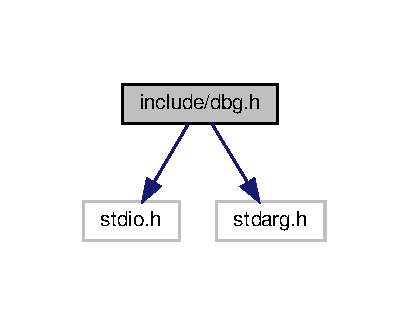
\includegraphics[width=196pt]{dbg_8h__incl}
\end{center}
\end{figure}
\subsection*{Macros}
\begin{DoxyCompactItemize}
\item 
\mbox{\Hypertarget{dbg_8h_a96dd473db0b3d10bd43390cdacb00120}\label{dbg_8h_a96dd473db0b3d10bd43390cdacb00120}} 
\#define {\bfseries D\+E\+B\+UG}(...)~D\+E\+B\+U\+G\+\_\+\+F\+U\+NC(\+\_\+\+\_\+\+F\+I\+L\+E\+\_\+\+\_\+, \+\_\+\+\_\+\+L\+I\+N\+E\+\_\+\+\_\+, \+\_\+\+\_\+\+V\+A\+\_\+\+A\+R\+G\+S\+\_\+\+\_\+)
\end{DoxyCompactItemize}
\subsection*{Functions}
\begin{DoxyCompactItemize}
\item 
\mbox{\Hypertarget{dbg_8h_ac308824d64d6bd9e803019f0a6e04888}\label{dbg_8h_ac308824d64d6bd9e803019f0a6e04888}} 
static void {\bfseries D\+E\+B\+U\+G\+\_\+\+F\+U\+NC} (char const $\ast$file, int line, char const $\ast$fmt,...)
\end{DoxyCompactItemize}


\subsection{Detailed Description}
Debug functions for A\+VR. 

\begin{DoxyAuthor}{Author}
Seth Girvan (Lord) 
\end{DoxyAuthor}

\hypertarget{dvl_8h}{}\section{include/dvl/dvl.h File Reference}
\label{dvl_8h}\index{include/dvl/dvl.\+h@{include/dvl/dvl.\+h}}


Interface function definitions for D\+VL.  


{\ttfamily \#include $<$stdbool.\+h$>$}\newline
Include dependency graph for dvl.\+h\+:\nopagebreak
\begin{figure}[H]
\begin{center}
\leavevmode
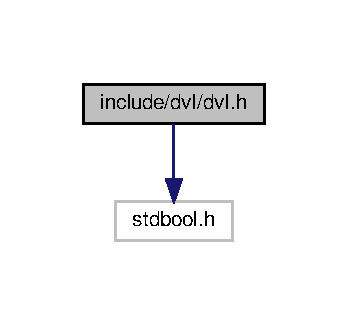
\includegraphics[width=167pt]{dvl_8h__incl}
\end{center}
\end{figure}
\subsection*{Functions}
\begin{DoxyCompactItemize}
\item 
\mbox{\Hypertarget{dvl_8h_ace13fbd095b6f793b7704a717902cef2}\label{dvl_8h_ace13fbd095b6f793b7704a717902cef2}} 
void \hyperlink{dvl_8h_ace13fbd095b6f793b7704a717902cef2}{dvl\+\_\+set\+\_\+data\+\_\+format} ()
\begin{DoxyCompactList}\small\item\em Configures proper D\+VL data components. \end{DoxyCompactList}\item 
\mbox{\Hypertarget{dvl_8h_a88885ad4d9407ea44a0d1473c85e459b}\label{dvl_8h_a88885ad4d9407ea44a0d1473c85e459b}} 
void \hyperlink{dvl_8h_a88885ad4d9407ea44a0d1473c85e459b}{dvl\+\_\+begin\+\_\+pinging} ()
\begin{DoxyCompactList}\small\item\em Tells D\+VL to begin pinging. \end{DoxyCompactList}\item 
\mbox{\Hypertarget{dvl_8h_a3e2d1045f92e30c7f8e21d2c54af5d8d}\label{dvl_8h_a3e2d1045f92e30c7f8e21d2c54af5d8d}} 
void \hyperlink{dvl_8h_a3e2d1045f92e30c7f8e21d2c54af5d8d}{reset\+\_\+parser} ()
\begin{DoxyCompactList}\small\item\em Discards the datagram that is being parsed. \end{DoxyCompactList}\item 
bool \hyperlink{dvl_8h_acd282756a658fc5e2fe729d9684263d1}{dvl\+\_\+data\+\_\+update} ()
\begin{DoxyCompactList}\small\item\em Replaces old data on the D\+VL with new data. \end{DoxyCompactList}\item 
int32\+\_\+t \hyperlink{dvl_8h_a42627cfa581f9b51ed01025e5deaf16e}{dvl\+\_\+get\+\_\+starboard\+\_\+vel} ()
\begin{DoxyCompactList}\small\item\em Finds velocity over bottom towards starboard. \end{DoxyCompactList}\item 
int32\+\_\+t \hyperlink{dvl_8h_a836f3040e47b915729718c2cdd6a9064}{dvl\+\_\+get\+\_\+forward\+\_\+vel} ()
\begin{DoxyCompactList}\small\item\em Finds velocity over bottom towards bow. \end{DoxyCompactList}\item 
int32\+\_\+t \hyperlink{dvl_8h_a5e5bdfedb1dcd23f982911e43552dea0}{dvl\+\_\+get\+\_\+upward\+\_\+vel} ()
\begin{DoxyCompactList}\small\item\em Finds velocity over bottom towards surface. \end{DoxyCompactList}\item 
int32\+\_\+t \hyperlink{dvl_8h_a67d1828f6fe430d9e886609d6c258f10}{dvl\+\_\+get\+\_\+range\+\_\+to\+\_\+bottom} ()
\begin{DoxyCompactList}\small\item\em Finds distance to bottom. \end{DoxyCompactList}\item 
bool \hyperlink{dvl_8h_ae35718ff4c189bdaaf55edc0288ad7fe}{dvl\+\_\+receive\+\_\+handler} ()
\begin{DoxyCompactList}\small\item\em Parses and processes received data. \end{DoxyCompactList}\item 
int \hyperlink{dvl_8h_aee5f5ff835ae272fd7d1e1fb9bf347fb}{send\+\_\+command} (char $\ast$cmd, bool wait)
\begin{DoxyCompactList}\small\item\em Sends command for D\+VL to process. \end{DoxyCompactList}\end{DoxyCompactItemize}


\subsection{Detailed Description}
Interface function definitions for D\+VL. 

\begin{DoxyAuthor}{Author}
Timothy Kanarsky 

David Zhang 
\end{DoxyAuthor}


\subsection{Function Documentation}
\mbox{\Hypertarget{dvl_8h_acd282756a658fc5e2fe729d9684263d1}\label{dvl_8h_acd282756a658fc5e2fe729d9684263d1}} 
\index{dvl.\+h@{dvl.\+h}!dvl\+\_\+data\+\_\+update@{dvl\+\_\+data\+\_\+update}}
\index{dvl\+\_\+data\+\_\+update@{dvl\+\_\+data\+\_\+update}!dvl.\+h@{dvl.\+h}}
\subsubsection{\texorpdfstring{dvl\+\_\+data\+\_\+update()}{dvl\_data\_update()}}
{\footnotesize\ttfamily bool dvl\+\_\+data\+\_\+update (\begin{DoxyParamCaption}{ }\end{DoxyParamCaption})}



Replaces old data on the D\+VL with new data. 

\begin{DoxyReturn}{Returns}
True on success. 
\end{DoxyReturn}
\mbox{\Hypertarget{dvl_8h_a836f3040e47b915729718c2cdd6a9064}\label{dvl_8h_a836f3040e47b915729718c2cdd6a9064}} 
\index{dvl.\+h@{dvl.\+h}!dvl\+\_\+get\+\_\+forward\+\_\+vel@{dvl\+\_\+get\+\_\+forward\+\_\+vel}}
\index{dvl\+\_\+get\+\_\+forward\+\_\+vel@{dvl\+\_\+get\+\_\+forward\+\_\+vel}!dvl.\+h@{dvl.\+h}}
\subsubsection{\texorpdfstring{dvl\+\_\+get\+\_\+forward\+\_\+vel()}{dvl\_get\_forward\_vel()}}
{\footnotesize\ttfamily int32\+\_\+t dvl\+\_\+get\+\_\+forward\+\_\+vel (\begin{DoxyParamCaption}{ }\end{DoxyParamCaption})}



Finds velocity over bottom towards bow. 

\begin{DoxyReturn}{Returns}
Velocity as 32-\/bit integer in 1um/s. 
\end{DoxyReturn}
\mbox{\Hypertarget{dvl_8h_a67d1828f6fe430d9e886609d6c258f10}\label{dvl_8h_a67d1828f6fe430d9e886609d6c258f10}} 
\index{dvl.\+h@{dvl.\+h}!dvl\+\_\+get\+\_\+range\+\_\+to\+\_\+bottom@{dvl\+\_\+get\+\_\+range\+\_\+to\+\_\+bottom}}
\index{dvl\+\_\+get\+\_\+range\+\_\+to\+\_\+bottom@{dvl\+\_\+get\+\_\+range\+\_\+to\+\_\+bottom}!dvl.\+h@{dvl.\+h}}
\subsubsection{\texorpdfstring{dvl\+\_\+get\+\_\+range\+\_\+to\+\_\+bottom()}{dvl\_get\_range\_to\_bottom()}}
{\footnotesize\ttfamily int32\+\_\+t dvl\+\_\+get\+\_\+range\+\_\+to\+\_\+bottom (\begin{DoxyParamCaption}{ }\end{DoxyParamCaption})}



Finds distance to bottom. 

Should not be negative. (\+:P)

\begin{DoxyReturn}{Returns}
Distance as 32-\/bit integer in 0.\+1mm. 
\end{DoxyReturn}
\mbox{\Hypertarget{dvl_8h_a42627cfa581f9b51ed01025e5deaf16e}\label{dvl_8h_a42627cfa581f9b51ed01025e5deaf16e}} 
\index{dvl.\+h@{dvl.\+h}!dvl\+\_\+get\+\_\+starboard\+\_\+vel@{dvl\+\_\+get\+\_\+starboard\+\_\+vel}}
\index{dvl\+\_\+get\+\_\+starboard\+\_\+vel@{dvl\+\_\+get\+\_\+starboard\+\_\+vel}!dvl.\+h@{dvl.\+h}}
\subsubsection{\texorpdfstring{dvl\+\_\+get\+\_\+starboard\+\_\+vel()}{dvl\_get\_starboard\_vel()}}
{\footnotesize\ttfamily int32\+\_\+t dvl\+\_\+get\+\_\+starboard\+\_\+vel (\begin{DoxyParamCaption}{ }\end{DoxyParamCaption})}



Finds velocity over bottom towards starboard. 

\begin{DoxyReturn}{Returns}
Velocity as 32-\/bit integer in 1um/s. 
\end{DoxyReturn}
\mbox{\Hypertarget{dvl_8h_a5e5bdfedb1dcd23f982911e43552dea0}\label{dvl_8h_a5e5bdfedb1dcd23f982911e43552dea0}} 
\index{dvl.\+h@{dvl.\+h}!dvl\+\_\+get\+\_\+upward\+\_\+vel@{dvl\+\_\+get\+\_\+upward\+\_\+vel}}
\index{dvl\+\_\+get\+\_\+upward\+\_\+vel@{dvl\+\_\+get\+\_\+upward\+\_\+vel}!dvl.\+h@{dvl.\+h}}
\subsubsection{\texorpdfstring{dvl\+\_\+get\+\_\+upward\+\_\+vel()}{dvl\_get\_upward\_vel()}}
{\footnotesize\ttfamily int32\+\_\+t dvl\+\_\+get\+\_\+upward\+\_\+vel (\begin{DoxyParamCaption}{ }\end{DoxyParamCaption})}



Finds velocity over bottom towards surface. 

\begin{DoxyReturn}{Returns}
Velocity as 32-\/bit integer in 1um/s. 
\end{DoxyReturn}
\mbox{\Hypertarget{dvl_8h_ae35718ff4c189bdaaf55edc0288ad7fe}\label{dvl_8h_ae35718ff4c189bdaaf55edc0288ad7fe}} 
\index{dvl.\+h@{dvl.\+h}!dvl\+\_\+receive\+\_\+handler@{dvl\+\_\+receive\+\_\+handler}}
\index{dvl\+\_\+receive\+\_\+handler@{dvl\+\_\+receive\+\_\+handler}!dvl.\+h@{dvl.\+h}}
\subsubsection{\texorpdfstring{dvl\+\_\+receive\+\_\+handler()}{dvl\_receive\_handler()}}
{\footnotesize\ttfamily bool dvl\+\_\+receive\+\_\+handler (\begin{DoxyParamCaption}{ }\end{DoxyParamCaption})}



Parses and processes received data. 

\begin{DoxyReturn}{Returns}
True when a complete datagram has been parsed. 
\end{DoxyReturn}
\mbox{\Hypertarget{dvl_8h_aee5f5ff835ae272fd7d1e1fb9bf347fb}\label{dvl_8h_aee5f5ff835ae272fd7d1e1fb9bf347fb}} 
\index{dvl.\+h@{dvl.\+h}!send\+\_\+command@{send\+\_\+command}}
\index{send\+\_\+command@{send\+\_\+command}!dvl.\+h@{dvl.\+h}}
\subsubsection{\texorpdfstring{send\+\_\+command()}{send\_command()}}
{\footnotesize\ttfamily int send\+\_\+command (\begin{DoxyParamCaption}\item[{char $\ast$}]{cmd,  }\item[{bool}]{wait }\end{DoxyParamCaption})}



Sends command for D\+VL to process. 


\begin{DoxyParams}{Parameters}
{\em cmd} & The command as a character. \\
\hline
{\em wait} & If true, waits until D\+VL is finished processing before sending the command. \\
\hline
\end{DoxyParams}
\begin{DoxyReturn}{Returns}
1 on success, negative number on error. 
\end{DoxyReturn}

\hypertarget{dvl__commands_8h}{}\section{include/dvl/dvl\+\_\+commands.h File Reference}
\label{dvl__commands_8h}\index{include/dvl/dvl\+\_\+commands.\+h@{include/dvl/dvl\+\_\+commands.\+h}}


Interface function definitions for D\+VL.  


\subsection*{Macros}
\begin{DoxyCompactItemize}
\item 
\mbox{\Hypertarget{dvl__commands_8h_adef3034178d2e2de064a8709350e8f01}\label{dvl__commands_8h_adef3034178d2e2de064a8709350e8f01}} 
\#define {\bfseries N\+U\+M\+\_\+\+C\+O\+M\+M\+A\+N\+DS}~12
\end{DoxyCompactItemize}
\subsection*{Variables}
\begin{DoxyCompactItemize}
\item 
\mbox{\Hypertarget{dvl__commands_8h_a8fc19b86e102436b966cc32b5748ae72}\label{dvl__commands_8h_a8fc19b86e102436b966cc32b5748ae72}} 
char $\ast$ {\bfseries break\+\_\+command} = \char`\"{}===\char`\"{}
\item 
char $\ast$ \hyperlink{dvl__commands_8h_a4005b50caf69d0e6e2eb922578ef2850}{setup\+\_\+commands} \mbox{[}N\+U\+M\+\_\+\+C\+O\+M\+M\+A\+N\+DS\mbox{]}
\begin{DoxyCompactList}\small\item\em Important setup commands. \end{DoxyCompactList}\item 
\mbox{\Hypertarget{dvl__commands_8h_a727a7a096d28f9baa4605f2060612184}\label{dvl__commands_8h_a727a7a096d28f9baa4605f2060612184}} 
char $\ast$ {\bfseries ping\+\_\+command} = \char`\"{}cs\textbackslash{}r\char`\"{}
\end{DoxyCompactItemize}


\subsection{Detailed Description}
Interface function definitions for D\+VL. 

\begin{DoxyAuthor}{Author}
Timothy Kanarsky 
\end{DoxyAuthor}


\subsection{Variable Documentation}
\mbox{\Hypertarget{dvl__commands_8h_a4005b50caf69d0e6e2eb922578ef2850}\label{dvl__commands_8h_a4005b50caf69d0e6e2eb922578ef2850}} 
\index{dvl\+\_\+commands.\+h@{dvl\+\_\+commands.\+h}!setup\+\_\+commands@{setup\+\_\+commands}}
\index{setup\+\_\+commands@{setup\+\_\+commands}!dvl\+\_\+commands.\+h@{dvl\+\_\+commands.\+h}}
\subsubsection{\texorpdfstring{setup\+\_\+commands}{setup\_commands}}
{\footnotesize\ttfamily char$\ast$ setup\+\_\+commands\mbox{[}N\+U\+M\+\_\+\+C\+O\+M\+M\+A\+N\+DS\mbox{]}}

{\bfseries Initial value\+:}
\begin{DoxyCode}
= \{
    \textcolor{stringliteral}{"CR1\(\backslash\)r"}, 
    \textcolor{stringliteral}{"BX00100\(\backslash\)r"}, 
    \textcolor{stringliteral}{"#BJ000110000\(\backslash\)r"}, 
    \textcolor{stringliteral}{"CF11110\(\backslash\)r"}, 
    
    \textcolor{stringliteral}{"EA-04500\(\backslash\)r"}, 
    \textcolor{stringliteral}{"ED00010\(\backslash\)r"}, 



    \textcolor{stringliteral}{"ES00\(\backslash\)r"},

    \textcolor{stringliteral}{"EX01011\(\backslash\)r"},
    \textcolor{stringliteral}{"EZ10000010\(\backslash\)r"},
    \textcolor{stringliteral}{"#EU2\(\backslash\)r"},
    \textcolor{stringliteral}{"PA\(\backslash\)r"},
    \textcolor{stringliteral}{"CK\(\backslash\)r"}
\}
\end{DoxyCode}


Important setup commands. 

C\+R1 -\/ Resets D\+VL to factory settings B\+X00100 -\/ Sets max depth to 100dm (33ft) \#\+B\+J000110000 -\/ Enables high-\/res velocity and range output C\+F11110 -\/ Sets auto-\/ping, binary output EA -\/ Determine angle correction based on D\+VL mount angle. E\+A-\/04500 -\/ Determine the angle correction based on D\+VL mount angle. E\+D00010 -\/ Depth of transducer, set to 1m because it doesn\textquotesingle{}t matter too much. 
\hypertarget{io__dvl_8h}{}\section{include/dvl/io\+\_\+dvl.h File Reference}
\label{io__dvl_8h}\index{include/dvl/io\+\_\+dvl.\+h@{include/dvl/io\+\_\+dvl.\+h}}


Low-\/level communication function definitions for D\+VL.  


{\ttfamily \#include $<$stdio.\+h$>$}\newline
{\ttfamily \#include $<$stdbool.\+h$>$}\newline
Include dependency graph for io\+\_\+dvl.\+h\+:\nopagebreak
\begin{figure}[H]
\begin{center}
\leavevmode
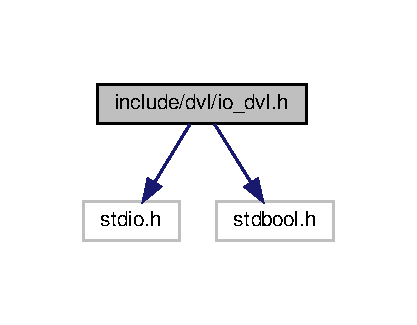
\includegraphics[width=200pt]{io__dvl_8h__incl}
\end{center}
\end{figure}
\subsection*{Functions}
\begin{DoxyCompactItemize}
\item 
void \hyperlink{io__dvl_8h_ab23125b4617e1730e49d0c4e837161d8}{io\+\_\+dvl\+\_\+init} (bool($\ast$recv\+\_\+handler)())
\begin{DoxyCompactList}\small\item\em Prepare D\+VL to receive data. \end{DoxyCompactList}\item 
\mbox{\Hypertarget{io__dvl_8h_a519393ef88a5185eed9b25f7473a80ca}\label{io__dvl_8h_a519393ef88a5185eed9b25f7473a80ca}} 
void \hyperlink{io__dvl_8h_a519393ef88a5185eed9b25f7473a80ca}{io\+\_\+dvl\+\_\+clean} ()
\begin{DoxyCompactList}\small\item\em Disable transmitting and receiving. \end{DoxyCompactList}\item 
\mbox{\Hypertarget{io__dvl_8h_aa7d789d7ecda6e4e626b33334bbbbd92}\label{io__dvl_8h_aa7d789d7ecda6e4e626b33334bbbbd92}} 
void \hyperlink{io__dvl_8h_aa7d789d7ecda6e4e626b33334bbbbd92}{io\+\_\+dvl\+\_\+recv\+\_\+begin} ()
\begin{DoxyCompactList}\small\item\em Tell D\+VL to begin sending data for us to receive. \end{DoxyCompactList}\item 
\mbox{\Hypertarget{io__dvl_8h_aed4a82bee0a703f2d95983c709a7da97}\label{io__dvl_8h_aed4a82bee0a703f2d95983c709a7da97}} 
void \hyperlink{io__dvl_8h_aed4a82bee0a703f2d95983c709a7da97}{io\+\_\+dvl\+\_\+recv\+\_\+end} ()
\begin{DoxyCompactList}\small\item\em Tell D\+VL to stop sending data. \end{DoxyCompactList}\item 
bool \hyperlink{io__dvl_8h_a938d90dc54f66989a252f968d7473aff}{io\+\_\+dvl\+\_\+tripbuf\+\_\+update} ()
\begin{DoxyCompactList}\small\item\em Updates tripbuf with new data if present. \end{DoxyCompactList}\item 
\mbox{\Hypertarget{io__dvl_8h_a592a6b73d2fec484a02af3a9bb4560ed}\label{io__dvl_8h_a592a6b73d2fec484a02af3a9bb4560ed}} 
void \hyperlink{io__dvl_8h_a592a6b73d2fec484a02af3a9bb4560ed}{io\+\_\+dvl\+\_\+tripbuf\+\_\+offer} ()
\begin{DoxyCompactList}\small\item\em Allows tripbuf to be written to again. \end{DoxyCompactList}\item 
unsigned char \hyperlink{io__dvl_8h_a1949eed459f94e0f3b521798df6f4cca}{io\+\_\+dvl\+\_\+tripbuf\+\_\+get\+\_\+read\+\_\+idx} ()
\begin{DoxyCompactList}\small\item\em Finds tripbuf index to read from. \end{DoxyCompactList}\item 
unsigned char \hyperlink{io__dvl_8h_a0869111c36770cdabc6c2172734aaea2}{io\+\_\+dvl\+\_\+tripbuf\+\_\+get\+\_\+write\+\_\+idx} ()
\begin{DoxyCompactList}\small\item\em Finds tripbuf index to write to. \end{DoxyCompactList}\end{DoxyCompactItemize}
\subsection*{Variables}
\begin{DoxyCompactItemize}
\item 
\mbox{\Hypertarget{io__dvl_8h_ad4f717cd1276a18e3b35940fd9242569}\label{io__dvl_8h_ad4f717cd1276a18e3b35940fd9242569}} 
F\+I\+LE $\ast$ \hyperlink{io__dvl_8h_ad4f717cd1276a18e3b35940fd9242569}{io\+\_\+dvl}
\begin{DoxyCompactList}\small\item\em Handles communication to D\+VL using file stream format. \end{DoxyCompactList}\end{DoxyCompactItemize}


\subsection{Detailed Description}
Low-\/level communication function definitions for D\+VL. 

If attempting to understand D\+VL documentation, it is a good idea to look under A\+H\+RS as well, as the two are similar.

\begin{DoxyAuthor}{Author}
Timothy Kanarsky 
\end{DoxyAuthor}


\subsection{Function Documentation}
\mbox{\Hypertarget{io__dvl_8h_ab23125b4617e1730e49d0c4e837161d8}\label{io__dvl_8h_ab23125b4617e1730e49d0c4e837161d8}} 
\index{io\+\_\+dvl.\+h@{io\+\_\+dvl.\+h}!io\+\_\+dvl\+\_\+init@{io\+\_\+dvl\+\_\+init}}
\index{io\+\_\+dvl\+\_\+init@{io\+\_\+dvl\+\_\+init}!io\+\_\+dvl.\+h@{io\+\_\+dvl.\+h}}
\subsubsection{\texorpdfstring{io\+\_\+dvl\+\_\+init()}{io\_dvl\_init()}}
{\footnotesize\ttfamily void io\+\_\+dvl\+\_\+init (\begin{DoxyParamCaption}\item[{bool($\ast$)()}]{recv\+\_\+handler }\end{DoxyParamCaption})}



Prepare D\+VL to receive data. 


\begin{DoxyParams}{Parameters}
{\em recv\+\_\+handler} & Function that handles data received from D\+VL. \\
\hline
\end{DoxyParams}
\mbox{\Hypertarget{io__dvl_8h_a1949eed459f94e0f3b521798df6f4cca}\label{io__dvl_8h_a1949eed459f94e0f3b521798df6f4cca}} 
\index{io\+\_\+dvl.\+h@{io\+\_\+dvl.\+h}!io\+\_\+dvl\+\_\+tripbuf\+\_\+get\+\_\+read\+\_\+idx@{io\+\_\+dvl\+\_\+tripbuf\+\_\+get\+\_\+read\+\_\+idx}}
\index{io\+\_\+dvl\+\_\+tripbuf\+\_\+get\+\_\+read\+\_\+idx@{io\+\_\+dvl\+\_\+tripbuf\+\_\+get\+\_\+read\+\_\+idx}!io\+\_\+dvl.\+h@{io\+\_\+dvl.\+h}}
\subsubsection{\texorpdfstring{io\+\_\+dvl\+\_\+tripbuf\+\_\+get\+\_\+read\+\_\+idx()}{io\_dvl\_tripbuf\_get\_read\_idx()}}
{\footnotesize\ttfamily unsigned char io\+\_\+dvl\+\_\+tripbuf\+\_\+get\+\_\+read\+\_\+idx (\begin{DoxyParamCaption}{ }\end{DoxyParamCaption})}



Finds tripbuf index to read from. 

\begin{DoxyReturn}{Returns}
The index to read from. 
\end{DoxyReturn}
\mbox{\Hypertarget{io__dvl_8h_a0869111c36770cdabc6c2172734aaea2}\label{io__dvl_8h_a0869111c36770cdabc6c2172734aaea2}} 
\index{io\+\_\+dvl.\+h@{io\+\_\+dvl.\+h}!io\+\_\+dvl\+\_\+tripbuf\+\_\+get\+\_\+write\+\_\+idx@{io\+\_\+dvl\+\_\+tripbuf\+\_\+get\+\_\+write\+\_\+idx}}
\index{io\+\_\+dvl\+\_\+tripbuf\+\_\+get\+\_\+write\+\_\+idx@{io\+\_\+dvl\+\_\+tripbuf\+\_\+get\+\_\+write\+\_\+idx}!io\+\_\+dvl.\+h@{io\+\_\+dvl.\+h}}
\subsubsection{\texorpdfstring{io\+\_\+dvl\+\_\+tripbuf\+\_\+get\+\_\+write\+\_\+idx()}{io\_dvl\_tripbuf\_get\_write\_idx()}}
{\footnotesize\ttfamily unsigned char io\+\_\+dvl\+\_\+tripbuf\+\_\+get\+\_\+write\+\_\+idx (\begin{DoxyParamCaption}{ }\end{DoxyParamCaption})}



Finds tripbuf index to write to. 

\begin{DoxyReturn}{Returns}
The index to write from. 
\end{DoxyReturn}
\mbox{\Hypertarget{io__dvl_8h_a938d90dc54f66989a252f968d7473aff}\label{io__dvl_8h_a938d90dc54f66989a252f968d7473aff}} 
\index{io\+\_\+dvl.\+h@{io\+\_\+dvl.\+h}!io\+\_\+dvl\+\_\+tripbuf\+\_\+update@{io\+\_\+dvl\+\_\+tripbuf\+\_\+update}}
\index{io\+\_\+dvl\+\_\+tripbuf\+\_\+update@{io\+\_\+dvl\+\_\+tripbuf\+\_\+update}!io\+\_\+dvl.\+h@{io\+\_\+dvl.\+h}}
\subsubsection{\texorpdfstring{io\+\_\+dvl\+\_\+tripbuf\+\_\+update()}{io\_dvl\_tripbuf\_update()}}
{\footnotesize\ttfamily bool io\+\_\+dvl\+\_\+tripbuf\+\_\+update (\begin{DoxyParamCaption}{ }\end{DoxyParamCaption})}



Updates tripbuf with new data if present. 

\begin{DoxyReturn}{Returns}
Whether there has been new data since the last call. 
\end{DoxyReturn}

\hypertarget{io_8hpp}{}\section{include/io.hpp File Reference}
\label{io_8hpp}\index{include/io.\+hpp@{include/io.\+hpp}}


IO and kill switch function definitions.  


{\ttfamily \#include \char`\"{}motor.\+hpp\char`\"{}}\newline
{\ttfamily \#include \char`\"{}m5/m5.\+h\char`\"{}}\newline
{\ttfamily \#include \char`\"{}m5/io\+\_\+m5.\+h\char`\"{}}\newline
{\ttfamily \#include \char`\"{}io.\+hpp\char`\"{}}\newline
{\ttfamily \#include \char`\"{}servo.\+h\char`\"{}}\newline
Include dependency graph for io.\+hpp\+:
\nopagebreak
\begin{figure}[H]
\begin{center}
\leavevmode
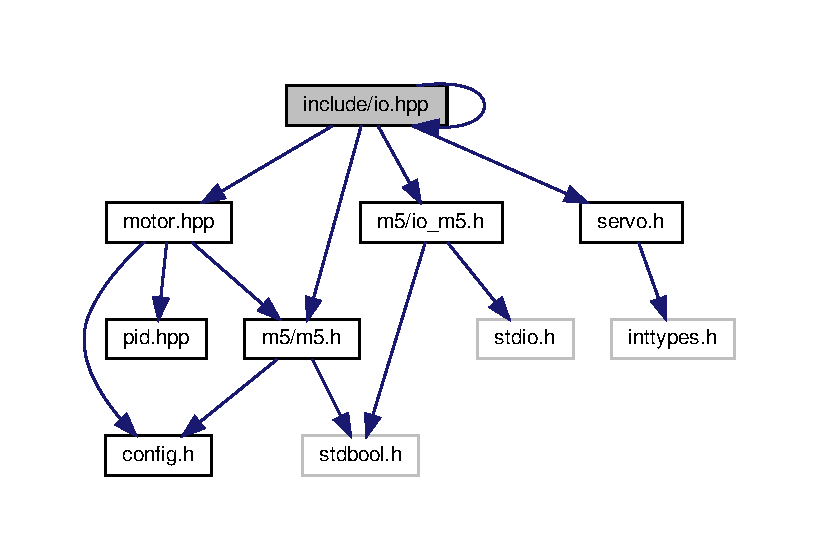
\includegraphics[width=350pt]{io_8hpp__incl}
\end{center}
\end{figure}
This graph shows which files directly or indirectly include this file\+:
\nopagebreak
\begin{figure}[H]
\begin{center}
\leavevmode
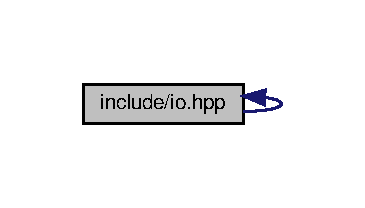
\includegraphics[width=175pt]{io_8hpp__dep__incl}
\end{center}
\end{figure}
\subsection*{Macros}
\begin{DoxyCompactItemize}
\item 
\mbox{\Hypertarget{io_8hpp_a27247678cfd6a8cb8b5a04d9c11053d7}\label{io_8hpp_a27247678cfd6a8cb8b5a04d9c11053d7}} 
\#define {\bfseries D\+E\+P\+T\+H\+\_\+\+P\+IN}~A0
\item 
\mbox{\Hypertarget{io_8hpp_aff1372f6d6eba317ecc336b8e4822963}\label{io_8hpp_aff1372f6d6eba317ecc336b8e4822963}} 
\#define {\bfseries K\+I\+L\+L\+\_\+\+P\+IN}~30
\end{DoxyCompactItemize}
\subsection*{Functions}
\begin{DoxyCompactItemize}
\item 
\mbox{\Hypertarget{io_8hpp_ac2651270fddbd8b61862729764f591fe}\label{io_8hpp_ac2651270fddbd8b61862729764f591fe}} 
void \hyperlink{io_8hpp_ac2651270fddbd8b61862729764f591fe}{io} ()
\begin{DoxyCompactList}\small\item\em Starts IO initialization for all major hardware (A\+H\+RS, D\+VL, M5, depth sensor, kill switch). \end{DoxyCompactList}\item 
void \hyperlink{io_8hpp_ae779516839d36e47d80e8faabfa03259}{drop} (int idx, int val)
\begin{DoxyCompactList}\small\item\em Turns servo to drop ball from dropper. \end{DoxyCompactList}\item 
bool \hyperlink{io_8hpp_a7c2ff3cdf102a2adb5ca47cb932acc9d}{alive} ()
\begin{DoxyCompactList}\small\item\em Reads kill state from the kill switch. \end{DoxyCompactList}\end{DoxyCompactItemize}
\subsection*{Variables}
\begin{DoxyCompactItemize}
\item 
\mbox{\Hypertarget{io_8hpp_a3e9350a91f7cb9ec3989955b454ef68e}\label{io_8hpp_a3e9350a91f7cb9ec3989955b454ef68e}} 
\hyperlink{classServoTimer2}{Servo\+Timer2} {\bfseries dropper1}
\item 
\mbox{\Hypertarget{io_8hpp_af6b1b58029f5269374c846cd1eadb70c}\label{io_8hpp_af6b1b58029f5269374c846cd1eadb70c}} 
\hyperlink{classServoTimer2}{Servo\+Timer2} {\bfseries dropper2}
\end{DoxyCompactItemize}


\subsection{Detailed Description}
IO and kill switch function definitions. 

\begin{DoxyAuthor}{Author}
David Zhang 
\end{DoxyAuthor}


\subsection{Function Documentation}
\mbox{\Hypertarget{io_8hpp_a7c2ff3cdf102a2adb5ca47cb932acc9d}\label{io_8hpp_a7c2ff3cdf102a2adb5ca47cb932acc9d}} 
\index{io.\+hpp@{io.\+hpp}!alive@{alive}}
\index{alive@{alive}!io.\+hpp@{io.\+hpp}}
\subsubsection{\texorpdfstring{alive()}{alive()}}
{\footnotesize\ttfamily bool alive (\begin{DoxyParamCaption}{ }\end{DoxyParamCaption})}



Reads kill state from the kill switch. 

\begin{DoxyReturn}{Returns}
True on alive. 
\end{DoxyReturn}
\mbox{\Hypertarget{io_8hpp_ae779516839d36e47d80e8faabfa03259}\label{io_8hpp_ae779516839d36e47d80e8faabfa03259}} 
\index{io.\+hpp@{io.\+hpp}!drop@{drop}}
\index{drop@{drop}!io.\+hpp@{io.\+hpp}}
\subsubsection{\texorpdfstring{drop()}{drop()}}
{\footnotesize\ttfamily void drop (\begin{DoxyParamCaption}\item[{int}]{idx,  }\item[{int}]{val }\end{DoxyParamCaption})}



Turns servo to drop ball from dropper. 


\begin{DoxyParams}{Parameters}
{\em idx} & 0 drops first servo, 1 drops second. \\
\hline
{\em val} & 0 means in, 1 means out. \\
\hline
\end{DoxyParams}

\hypertarget{kalman_8hpp}{}\section{include/kalman.hpp File Reference}
\label{kalman_8hpp}\index{include/kalman.\+hpp@{include/kalman.\+hpp}}


\hyperlink{structKalman}{Kalman} filter struct and constant definitions.  


\subsection*{Data Structures}
\begin{DoxyCompactItemize}
\item 
struct \hyperlink{structKalman}{Kalman}
\begin{DoxyCompactList}\small\item\em Struct to make using the \hyperlink{structKalman}{Kalman} filter easier. \end{DoxyCompactList}\end{DoxyCompactItemize}
\subsection*{Variables}
\begin{DoxyCompactItemize}
\item 
static const int \hyperlink{kalman_8hpp_ab2b6b0c222cd1ce70d6a831f57241e59}{N} = 6
\item 
\mbox{\Hypertarget{kalman_8hpp_a9edc6895d567e0ddcdd3cc20df3f3b4b}\label{kalman_8hpp_a9edc6895d567e0ddcdd3cc20df3f3b4b}} 
static const int {\bfseries M} = 2
\item 
static float \hyperlink{kalman_8hpp_a51c1d090ecb85f96345bb359da0c40d6}{Qk} \mbox{[}\hyperlink{kalman_8hpp_ab2b6b0c222cd1ce70d6a831f57241e59}{N} $\ast$\hyperlink{kalman_8hpp_ab2b6b0c222cd1ce70d6a831f57241e59}{N}\mbox{]}
\item 
static float \hyperlink{kalman_8hpp_aa70fba75014a727d78d8d3577de35beb}{Hk} \mbox{[}M $\ast$\hyperlink{kalman_8hpp_ab2b6b0c222cd1ce70d6a831f57241e59}{N}\mbox{]}
\item 
static float \hyperlink{kalman_8hpp_a211f44ae6253f79a609558455c4732e9}{Rk} \mbox{[}M $\ast$M\mbox{]}
\end{DoxyCompactItemize}


\subsection{Detailed Description}
\hyperlink{structKalman}{Kalman} filter struct and constant definitions. 

The state of the \hyperlink{structKalman}{Kalman} filter can be described by the following vector\+: \mbox{[}X VX AX Y VY AY\mbox{]}

The main measurement instrument used for this \hyperlink{structKalman}{Kalman} filter is a D\+VL, which returns VX and VY. The exact variances of the D\+VL are on the spreadsheet.

\begin{DoxyAuthor}{Author}
David Zhang 
\end{DoxyAuthor}


\subsection{Variable Documentation}
\mbox{\Hypertarget{kalman_8hpp_aa70fba75014a727d78d8d3577de35beb}\label{kalman_8hpp_aa70fba75014a727d78d8d3577de35beb}} 
\index{kalman.\+hpp@{kalman.\+hpp}!Hk@{Hk}}
\index{Hk@{Hk}!kalman.\+hpp@{kalman.\+hpp}}
\subsubsection{\texorpdfstring{Hk}{Hk}}
{\footnotesize\ttfamily float Hk\mbox{[}M $\ast$\hyperlink{kalman_8hpp_ab2b6b0c222cd1ce70d6a831f57241e59}{N}\mbox{]}\hspace{0.3cm}{\ttfamily [static]}}

{\bfseries Initial value\+:}
\begin{DoxyCode}
= \{
    0.000, 1.000, 0.000, 0.000, 0.000, 0.000,
    0.000, 0.000, 0.000, 0.000, 1.000, 0.000
\}
\end{DoxyCode}
Hk maps the predicted state to measurements. \mbox{\Hypertarget{kalman_8hpp_ab2b6b0c222cd1ce70d6a831f57241e59}\label{kalman_8hpp_ab2b6b0c222cd1ce70d6a831f57241e59}} 
\index{kalman.\+hpp@{kalman.\+hpp}!N@{N}}
\index{N@{N}!kalman.\+hpp@{kalman.\+hpp}}
\subsubsection{\texorpdfstring{N}{N}}
{\footnotesize\ttfamily const int N = 6\hspace{0.3cm}{\ttfamily [static]}}

N represents the number of elements in the state, while M represents the number of sensors. \mbox{\Hypertarget{kalman_8hpp_a51c1d090ecb85f96345bb359da0c40d6}\label{kalman_8hpp_a51c1d090ecb85f96345bb359da0c40d6}} 
\index{kalman.\+hpp@{kalman.\+hpp}!Qk@{Qk}}
\index{Qk@{Qk}!kalman.\+hpp@{kalman.\+hpp}}
\subsubsection{\texorpdfstring{Qk}{Qk}}
{\footnotesize\ttfamily float Qk\mbox{[}\hyperlink{kalman_8hpp_ab2b6b0c222cd1ce70d6a831f57241e59}{N} $\ast$\hyperlink{kalman_8hpp_ab2b6b0c222cd1ce70d6a831f57241e59}{N}\mbox{]}\hspace{0.3cm}{\ttfamily [static]}}

{\bfseries Initial value\+:}
\begin{DoxyCode}
= \{
    0.005, 0.000, 0.000, 0.000, 0.000, 0.000,
    0.000, 0.005, 0.000, 0.000, 0.000, 0.000,
    0.000, 0.000, 0.005, 0.000, 0.000, 0.000,
    0.000, 0.000, 0.000, 0.005, 0.000, 0.000,
    0.000, 0.000, 0.000, 0.000, 0.005, 0.000,
    0.000, 0.000, 0.000, 0.000, 0.000, 0.005
\}
\end{DoxyCode}
Qk describes how accurate the model is. The variance of each element of the should be along the main diagonal of the matrix. \mbox{\Hypertarget{kalman_8hpp_a211f44ae6253f79a609558455c4732e9}\label{kalman_8hpp_a211f44ae6253f79a609558455c4732e9}} 
\index{kalman.\+hpp@{kalman.\+hpp}!Rk@{Rk}}
\index{Rk@{Rk}!kalman.\+hpp@{kalman.\+hpp}}
\subsubsection{\texorpdfstring{Rk}{Rk}}
{\footnotesize\ttfamily float Rk\mbox{[}M $\ast$M\mbox{]}\hspace{0.3cm}{\ttfamily [static]}}

{\bfseries Initial value\+:}
\begin{DoxyCode}
= \{
    5.000, 0.000,
    0.000, 5.000
\}
\end{DoxyCode}
Rk describes the precision of each measurement. 
\hypertarget{crc32_8h}{}\section{include/m5/crc32.h File Reference}
\label{crc32_8h}\index{include/m5/crc32.\+h@{include/m5/crc32.\+h}}


Helper functions for C\+RC.  


{\ttfamily \#include $<$stdint.\+h$>$}\newline
Include dependency graph for crc32.\+h\+:\nopagebreak
\begin{figure}[H]
\begin{center}
\leavevmode
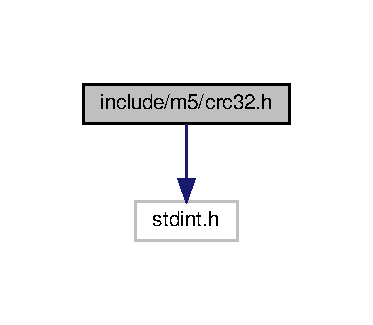
\includegraphics[width=179pt]{crc32_8h__incl}
\end{center}
\end{figure}
\subsection*{Macros}
\begin{DoxyCompactItemize}
\item 
\#define \hyperlink{crc32_8h_a6d8ef42a00579f2a84aca31d587e012d}{C\+R\+C32\+\_\+\+I\+N\+I\+T\+\_\+\+S\+E\+ED}~((uint32\+\_\+t)0x\+F\+F\+F\+F\+F\+F\+F\+F)
\item 
\#define \hyperlink{crc32_8h_a8e74c976f75a347418553cf36c5573fe}{C\+R\+C32\+\_\+\+L\+E\+\_\+\+R\+E\+S\+I\+D\+UE}~((uint32\+\_\+t)0x2144\+D\+F1\+C)
\end{DoxyCompactItemize}
\subsection*{Functions}
\begin{DoxyCompactItemize}
\item 
uint32\+\_\+t \hyperlink{crc32_8h_a24d6fe2ac5fe0403bc92b23d82533164}{crc32\+\_\+update} (uint32\+\_\+t crc, uint8\+\_\+t data)
\begin{DoxyCompactList}\small\item\em Updates a C\+RC with a byte of data. \end{DoxyCompactList}\item 
uint32\+\_\+t \hyperlink{crc32_8h_ab31566d3a4b466db0623254d02b8d5a5}{crc32\+\_\+final\+\_\+mask} (uint32\+\_\+t crc)
\begin{DoxyCompactList}\small\item\em Applies a final X\+OR mask to a C\+RC. (0x\+F\+F\+F\+F\+F\+F\+FF) \end{DoxyCompactList}\end{DoxyCompactItemize}


\subsection{Detailed Description}
Helper functions for C\+RC. 

\begin{DoxyAuthor}{Author}
Seth Girvan (Lord) 
\end{DoxyAuthor}


\subsection{Macro Definition Documentation}
\mbox{\Hypertarget{crc32_8h_a6d8ef42a00579f2a84aca31d587e012d}\label{crc32_8h_a6d8ef42a00579f2a84aca31d587e012d}} 
\index{crc32.\+h@{crc32.\+h}!C\+R\+C32\+\_\+\+I\+N\+I\+T\+\_\+\+S\+E\+ED@{C\+R\+C32\+\_\+\+I\+N\+I\+T\+\_\+\+S\+E\+ED}}
\index{C\+R\+C32\+\_\+\+I\+N\+I\+T\+\_\+\+S\+E\+ED@{C\+R\+C32\+\_\+\+I\+N\+I\+T\+\_\+\+S\+E\+ED}!crc32.\+h@{crc32.\+h}}
\subsubsection{\texorpdfstring{C\+R\+C32\+\_\+\+I\+N\+I\+T\+\_\+\+S\+E\+ED}{CRC32\_INIT\_SEED}}
{\footnotesize\ttfamily \#define C\+R\+C32\+\_\+\+I\+N\+I\+T\+\_\+\+S\+E\+ED~((uint32\+\_\+t)0x\+F\+F\+F\+F\+F\+F\+F\+F)}

Implements the A\+N\+SI X3.\+66 32 bit cyclic reduncy check.\+Pass to \hyperlink{crc32_8h_a24d6fe2ac5fe0403bc92b23d82533164}{crc32\+\_\+update()} as arg crc with the first byte of data. \mbox{\Hypertarget{crc32_8h_a8e74c976f75a347418553cf36c5573fe}\label{crc32_8h_a8e74c976f75a347418553cf36c5573fe}} 
\index{crc32.\+h@{crc32.\+h}!C\+R\+C32\+\_\+\+L\+E\+\_\+\+R\+E\+S\+I\+D\+UE@{C\+R\+C32\+\_\+\+L\+E\+\_\+\+R\+E\+S\+I\+D\+UE}}
\index{C\+R\+C32\+\_\+\+L\+E\+\_\+\+R\+E\+S\+I\+D\+UE@{C\+R\+C32\+\_\+\+L\+E\+\_\+\+R\+E\+S\+I\+D\+UE}!crc32.\+h@{crc32.\+h}}
\subsubsection{\texorpdfstring{C\+R\+C32\+\_\+\+L\+E\+\_\+\+R\+E\+S\+I\+D\+UE}{CRC32\_LE\_RESIDUE}}
{\footnotesize\ttfamily \#define C\+R\+C32\+\_\+\+L\+E\+\_\+\+R\+E\+S\+I\+D\+UE~((uint32\+\_\+t)0x2144\+D\+F1\+C)}

The C\+R\+C32 of any value with its little endian C\+R\+C32 appended. 

\subsection{Function Documentation}
\mbox{\Hypertarget{crc32_8h_ab31566d3a4b466db0623254d02b8d5a5}\label{crc32_8h_ab31566d3a4b466db0623254d02b8d5a5}} 
\index{crc32.\+h@{crc32.\+h}!crc32\+\_\+final\+\_\+mask@{crc32\+\_\+final\+\_\+mask}}
\index{crc32\+\_\+final\+\_\+mask@{crc32\+\_\+final\+\_\+mask}!crc32.\+h@{crc32.\+h}}
\subsubsection{\texorpdfstring{crc32\+\_\+final\+\_\+mask()}{crc32\_final\_mask()}}
{\footnotesize\ttfamily uint32\+\_\+t crc32\+\_\+final\+\_\+mask (\begin{DoxyParamCaption}\item[{uint32\+\_\+t}]{crc }\end{DoxyParamCaption})}



Applies a final X\+OR mask to a C\+RC. (0x\+F\+F\+F\+F\+F\+F\+FF) 

Should be done after \hyperlink{crc32_8h_a24d6fe2ac5fe0403bc92b23d82533164}{crc32\+\_\+update()} has been called for all data.


\begin{DoxyParams}{Parameters}
{\em crc} & C\+RC that receives the mask. \\
\hline
\end{DoxyParams}
\begin{DoxyReturn}{Returns}
New C\+RC after the mask. 
\end{DoxyReturn}
\mbox{\Hypertarget{crc32_8h_a24d6fe2ac5fe0403bc92b23d82533164}\label{crc32_8h_a24d6fe2ac5fe0403bc92b23d82533164}} 
\index{crc32.\+h@{crc32.\+h}!crc32\+\_\+update@{crc32\+\_\+update}}
\index{crc32\+\_\+update@{crc32\+\_\+update}!crc32.\+h@{crc32.\+h}}
\subsubsection{\texorpdfstring{crc32\+\_\+update()}{crc32\_update()}}
{\footnotesize\ttfamily uint32\+\_\+t crc32\+\_\+update (\begin{DoxyParamCaption}\item[{uint32\+\_\+t}]{crc,  }\item[{uint8\+\_\+t}]{data }\end{DoxyParamCaption})}



Updates a C\+RC with a byte of data. 

Wikipedia on C\+RC\+: \href{https://en.wikipedia.org/wiki/Cyclic_Redundancy_Check}{\tt https\+://en.\+wikipedia.\+org/wiki/\+Cyclic\+\_\+\+Redundancy\+\_\+\+Check}


\begin{DoxyParams}{Parameters}
{\em crc} & C\+RC to update. \\
\hline
{\em data} & Data to update C\+RC with. \\
\hline
\end{DoxyParams}
\begin{DoxyReturn}{Returns}
New C\+RC updated with data.
\end{DoxyReturn}
N\+O\+TE\+: An optimization would be to use a lookup-\/table implementation instead (with the table in flash on the avr). 
\hypertarget{io__m5_8h}{}\section{include/m5/io\+\_\+m5.h File Reference}
\label{io__m5_8h}\index{include/m5/io\+\_\+m5.\+h@{include/m5/io\+\_\+m5.\+h}}


Low-\/level communication function definitions for Videoray M5 motors.  


{\ttfamily \#include $<$stdio.\+h$>$}\newline
{\ttfamily \#include $<$stdbool.\+h$>$}\newline
Include dependency graph for io\+\_\+m5.\+h\+:\nopagebreak
\begin{figure}[H]
\begin{center}
\leavevmode
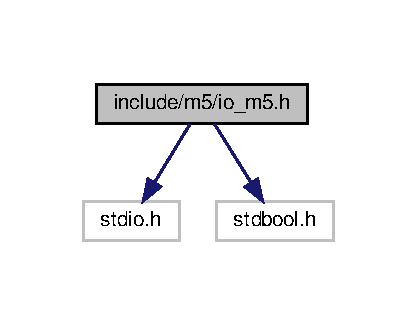
\includegraphics[width=200pt]{io__m5_8h__incl}
\end{center}
\end{figure}
This graph shows which files directly or indirectly include this file\+:
\nopagebreak
\begin{figure}[H]
\begin{center}
\leavevmode
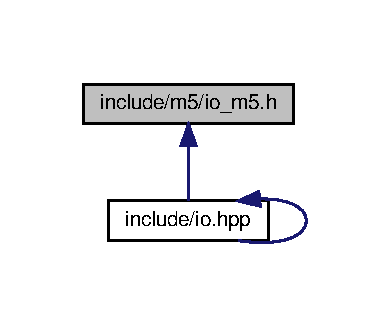
\includegraphics[width=187pt]{io__m5_8h__dep__incl}
\end{center}
\end{figure}
\subsection*{Functions}
\begin{DoxyCompactItemize}
\item 
void \hyperlink{io__m5_8h_ad572b5e5dccab0f1c5a962e08ce2912e}{io\+\_\+m5\+\_\+init} (char const $\ast$path)
\begin{DoxyCompactList}\small\item\em Prepare M5 motors to receive data. \end{DoxyCompactList}\item 
void \hyperlink{io__m5_8h_a57552be4efd362dfbaba37809d1f129d}{io\+\_\+m5\+\_\+clean} ()
\begin{DoxyCompactList}\small\item\em Disable transmitting and receiving. \end{DoxyCompactList}\item 
int \hyperlink{io__m5_8h_a515c36e7074c3d8f2a707f4dba147dd6}{io\+\_\+m5\+\_\+trans\+\_\+set} (int($\ast$handler)())
\begin{DoxyCompactList}\small\item\em Tell M5 motors to start receiving data. \end{DoxyCompactList}\item 
void \hyperlink{io__m5_8h_ab00f04dfb16c64ae321fc5294371b749}{io\+\_\+m5\+\_\+trans\+\_\+trywait} ()
\begin{DoxyCompactList}\small\item\em Suspends data transmission until there is new data. \end{DoxyCompactList}\item 
\mbox{\Hypertarget{io__m5_8h_a1297a12a88e41ab13442adb9bcace56d}\label{io__m5_8h_a1297a12a88e41ab13442adb9bcace56d}} 
void \hyperlink{io__m5_8h_a1297a12a88e41ab13442adb9bcace56d}{io\+\_\+m5\+\_\+trans\+\_\+stop} ()
\begin{DoxyCompactList}\small\item\em Stops motors until resume is called. \end{DoxyCompactList}\item 
bool \hyperlink{io__m5_8h_a0c610858e0abe25cf8e34076675ad623}{io\+\_\+m5\+\_\+tripbuf\+\_\+update} ()
\begin{DoxyCompactList}\small\item\em Updates tripbuf with new data. \end{DoxyCompactList}\item 
void \hyperlink{io__m5_8h_a9f3c3159f49e3e0d4532b3d535a9184d}{io\+\_\+m5\+\_\+tripbuf\+\_\+offer\+\_\+resume} ()
\begin{DoxyCompactList}\small\item\em Resumes motors after stopping. \end{DoxyCompactList}\item 
unsigned char \hyperlink{io__m5_8h_a17801e5afc9dfb2e05f1e96163cb2e84}{io\+\_\+m5\+\_\+tripbuf\+\_\+read} ()
\begin{DoxyCompactList}\small\item\em Finds the tripbuf index to read from. \end{DoxyCompactList}\item 
unsigned char \hyperlink{io__m5_8h_a202b3ed317ffca6c49d8e70e7ba0d7a7}{io\+\_\+m5\+\_\+tripbuf\+\_\+write} ()
\begin{DoxyCompactList}\small\item\em Finds the tripbuf index to write to. \end{DoxyCompactList}\end{DoxyCompactItemize}
\subsection*{Variables}
\begin{DoxyCompactItemize}
\item 
F\+I\+LE $\ast$ \hyperlink{io__m5_8h_ac3eb02f1b9ff9632d44f0f20a8b18e2e}{io\+\_\+m5}
\end{DoxyCompactItemize}


\subsection{Detailed Description}
Low-\/level communication function definitions for Videoray M5 motors. 

\begin{DoxyAuthor}{Author}
Seth Girvan (Lord) 
\end{DoxyAuthor}


\subsection{Function Documentation}
\mbox{\Hypertarget{io__m5_8h_a57552be4efd362dfbaba37809d1f129d}\label{io__m5_8h_a57552be4efd362dfbaba37809d1f129d}} 
\index{io\+\_\+m5.\+h@{io\+\_\+m5.\+h}!io\+\_\+m5\+\_\+clean@{io\+\_\+m5\+\_\+clean}}
\index{io\+\_\+m5\+\_\+clean@{io\+\_\+m5\+\_\+clean}!io\+\_\+m5.\+h@{io\+\_\+m5.\+h}}
\subsubsection{\texorpdfstring{io\+\_\+m5\+\_\+clean()}{io\_m5\_clean()}}
{\footnotesize\ttfamily void io\+\_\+m5\+\_\+clean (\begin{DoxyParamCaption}{ }\end{DoxyParamCaption})}



Disable transmitting and receiving. 

Unimplemented. \mbox{\Hypertarget{io__m5_8h_ad572b5e5dccab0f1c5a962e08ce2912e}\label{io__m5_8h_ad572b5e5dccab0f1c5a962e08ce2912e}} 
\index{io\+\_\+m5.\+h@{io\+\_\+m5.\+h}!io\+\_\+m5\+\_\+init@{io\+\_\+m5\+\_\+init}}
\index{io\+\_\+m5\+\_\+init@{io\+\_\+m5\+\_\+init}!io\+\_\+m5.\+h@{io\+\_\+m5.\+h}}
\subsubsection{\texorpdfstring{io\+\_\+m5\+\_\+init()}{io\_m5\_init()}}
{\footnotesize\ttfamily void io\+\_\+m5\+\_\+init (\begin{DoxyParamCaption}\item[{char const $\ast$}]{path }\end{DoxyParamCaption})}



Prepare M5 motors to receive data. 


\begin{DoxyParams}{Parameters}
{\em path} & Location of the motors, unused at the moment. \\
\hline
\end{DoxyParams}
\mbox{\Hypertarget{io__m5_8h_a515c36e7074c3d8f2a707f4dba147dd6}\label{io__m5_8h_a515c36e7074c3d8f2a707f4dba147dd6}} 
\index{io\+\_\+m5.\+h@{io\+\_\+m5.\+h}!io\+\_\+m5\+\_\+trans\+\_\+set@{io\+\_\+m5\+\_\+trans\+\_\+set}}
\index{io\+\_\+m5\+\_\+trans\+\_\+set@{io\+\_\+m5\+\_\+trans\+\_\+set}!io\+\_\+m5.\+h@{io\+\_\+m5.\+h}}
\subsubsection{\texorpdfstring{io\+\_\+m5\+\_\+trans\+\_\+set()}{io\_m5\_trans\_set()}}
{\footnotesize\ttfamily int io\+\_\+m5\+\_\+trans\+\_\+set (\begin{DoxyParamCaption}\item[{int($\ast$)()}]{handler }\end{DoxyParamCaption})}



Tell M5 motors to start receiving data. 

Asynchronous (concurrent on pc) data writing. It will not be started until io\+\_\+m5\+\_\+offer\+\_\+resume is called.


\begin{DoxyParams}{Parameters}
{\em Function} & that handles writing data to M5s. \\
\hline
\end{DoxyParams}
\mbox{\Hypertarget{io__m5_8h_ab00f04dfb16c64ae321fc5294371b749}\label{io__m5_8h_ab00f04dfb16c64ae321fc5294371b749}} 
\index{io\+\_\+m5.\+h@{io\+\_\+m5.\+h}!io\+\_\+m5\+\_\+trans\+\_\+trywait@{io\+\_\+m5\+\_\+trans\+\_\+trywait}}
\index{io\+\_\+m5\+\_\+trans\+\_\+trywait@{io\+\_\+m5\+\_\+trans\+\_\+trywait}!io\+\_\+m5.\+h@{io\+\_\+m5.\+h}}
\subsubsection{\texorpdfstring{io\+\_\+m5\+\_\+trans\+\_\+trywait()}{io\_m5\_trans\_trywait()}}
{\footnotesize\ttfamily void io\+\_\+m5\+\_\+trans\+\_\+trywait (\begin{DoxyParamCaption}{ }\end{DoxyParamCaption})}



Suspends data transmission until there is new data. 

To be called from the transmission handler (ie io\+\_\+m5\+\_\+trans\+\_\+set argument). Meant to be called after finishing transmission of a packet.

If io\+\_\+m5\+\_\+tripbuf\+\_\+offer\+\_\+resume has not been called since the last call of io\+\_\+m5\+\_\+tripbuf\+\_\+update, then the transmission handler is suspended for $\sim$.5 seconds or until io\+\_\+m5\+\_\+offer\+\_\+resume is called, whichever is first. If there is new triple buffer data available, returns immediately.

By default, a thruster will automatically set itself to power 0 if it has not received a command for over a second. While this can be disabled, it provides useful safety in case something goes fatally wrong in our software or there are connection problems. We could just transmit continuously (on the avr, never disabling the Data Register Ready Interrupt, but at 115,200 baud, that is a lot of processing wasted on the interrupt). While could probably just rely on io\+\_\+m5\+\_\+trans\+\_\+offer\+\_\+resume being called at least once a second, this times out after .5 seconds (arbitrary margin of safety) just in case.

Should only be called from handler\+\_\+m5\+\_\+trans. \mbox{\Hypertarget{io__m5_8h_a9f3c3159f49e3e0d4532b3d535a9184d}\label{io__m5_8h_a9f3c3159f49e3e0d4532b3d535a9184d}} 
\index{io\+\_\+m5.\+h@{io\+\_\+m5.\+h}!io\+\_\+m5\+\_\+tripbuf\+\_\+offer\+\_\+resume@{io\+\_\+m5\+\_\+tripbuf\+\_\+offer\+\_\+resume}}
\index{io\+\_\+m5\+\_\+tripbuf\+\_\+offer\+\_\+resume@{io\+\_\+m5\+\_\+tripbuf\+\_\+offer\+\_\+resume}!io\+\_\+m5.\+h@{io\+\_\+m5.\+h}}
\subsubsection{\texorpdfstring{io\+\_\+m5\+\_\+tripbuf\+\_\+offer\+\_\+resume()}{io\_m5\_tripbuf\_offer\_resume()}}
{\footnotesize\ttfamily void io\+\_\+m5\+\_\+tripbuf\+\_\+offer\+\_\+resume (\begin{DoxyParamCaption}{ }\end{DoxyParamCaption})}



Resumes motors after stopping. 

Makes the current write index available to io\+\_\+m5\+\_\+tripbuf\+\_\+update, and changes the value returned by io\+\_\+m5\+\_\+tripbuf\+\_\+write.

Every value in the write triple buffer (eg buf\mbox{[}\hyperlink{io__m5_8h_a202b3ed317ffca6c49d8e70e7ba0d7a7}{io\+\_\+m5\+\_\+tripbuf\+\_\+write()}\mbox{]} ) should be written before calling this, as unwritten areas have unspecified value.

Also resumes the transmission handler if it is paused (so it will start transmitting the new data asap). io\+\_\+m5\+\_\+trans\+\_\+set must be called before this is called.

May be interrupted by io\+\_\+m5\+\_\+tripbuf\+\_\+update, but must not interrupt it.

Always leaves the U\+S\+A\+RT Data Register Empty Interrupt Enabled. \mbox{\Hypertarget{io__m5_8h_a17801e5afc9dfb2e05f1e96163cb2e84}\label{io__m5_8h_a17801e5afc9dfb2e05f1e96163cb2e84}} 
\index{io\+\_\+m5.\+h@{io\+\_\+m5.\+h}!io\+\_\+m5\+\_\+tripbuf\+\_\+read@{io\+\_\+m5\+\_\+tripbuf\+\_\+read}}
\index{io\+\_\+m5\+\_\+tripbuf\+\_\+read@{io\+\_\+m5\+\_\+tripbuf\+\_\+read}!io\+\_\+m5.\+h@{io\+\_\+m5.\+h}}
\subsubsection{\texorpdfstring{io\+\_\+m5\+\_\+tripbuf\+\_\+read()}{io\_m5\_tripbuf\_read()}}
{\footnotesize\ttfamily unsigned char io\+\_\+m5\+\_\+tripbuf\+\_\+read (\begin{DoxyParamCaption}{ }\end{DoxyParamCaption})}



Finds the tripbuf index to read from. 

\begin{DoxyReturn}{Returns}
The index of the buffer the data consumer should read from. Only changes if io\+\_\+m5\+\_\+tripbuf\+\_\+update is called and returns true. 
\end{DoxyReturn}
\mbox{\Hypertarget{io__m5_8h_a0c610858e0abe25cf8e34076675ad623}\label{io__m5_8h_a0c610858e0abe25cf8e34076675ad623}} 
\index{io\+\_\+m5.\+h@{io\+\_\+m5.\+h}!io\+\_\+m5\+\_\+tripbuf\+\_\+update@{io\+\_\+m5\+\_\+tripbuf\+\_\+update}}
\index{io\+\_\+m5\+\_\+tripbuf\+\_\+update@{io\+\_\+m5\+\_\+tripbuf\+\_\+update}!io\+\_\+m5.\+h@{io\+\_\+m5.\+h}}
\subsubsection{\texorpdfstring{io\+\_\+m5\+\_\+tripbuf\+\_\+update()}{io\_m5\_tripbuf\_update()}}
{\footnotesize\ttfamily bool io\+\_\+m5\+\_\+tripbuf\+\_\+update (\begin{DoxyParamCaption}{ }\end{DoxyParamCaption})}



Updates tripbuf with new data. 

Causes io\+\_\+m5\+\_\+tripbuf\+\_\+read to return index that was most recently \textquotesingle{}submitted\textquotesingle{} by io\+\_\+m5\+\_\+tripbuf\+\_\+offer\+\_\+resume.

This should only be run between complete \textquotesingle{}uses\textquotesingle{} of the data, to avoid using disparate data.

Unfortunately, since there is no way to have a lock-\/free/interruptible triple buffer implementation on the avr, this has to be platform-\/specific. A lock-\/free ring buffer would not handle cases when the producer is faster than the consumer well.

\begin{DoxyReturn}{Returns}
True only if io\+\_\+m5\+\_\+tripbuf\+\_\+offer\+\_\+resume has been called (ie there is new data) since last call. 
\end{DoxyReturn}
\mbox{\Hypertarget{io__m5_8h_a202b3ed317ffca6c49d8e70e7ba0d7a7}\label{io__m5_8h_a202b3ed317ffca6c49d8e70e7ba0d7a7}} 
\index{io\+\_\+m5.\+h@{io\+\_\+m5.\+h}!io\+\_\+m5\+\_\+tripbuf\+\_\+write@{io\+\_\+m5\+\_\+tripbuf\+\_\+write}}
\index{io\+\_\+m5\+\_\+tripbuf\+\_\+write@{io\+\_\+m5\+\_\+tripbuf\+\_\+write}!io\+\_\+m5.\+h@{io\+\_\+m5.\+h}}
\subsubsection{\texorpdfstring{io\+\_\+m5\+\_\+tripbuf\+\_\+write()}{io\_m5\_tripbuf\_write()}}
{\footnotesize\ttfamily unsigned char io\+\_\+m5\+\_\+tripbuf\+\_\+write (\begin{DoxyParamCaption}{ }\end{DoxyParamCaption})}



Finds the tripbuf index to write to. 

\begin{DoxyReturn}{Returns}
The index of the buffer the data producer should write to. Only changes when io\+\_\+m5\+\_\+tripbuf\+\_\+offer\+\_\+resume is called. 
\end{DoxyReturn}


\subsection{Variable Documentation}
\mbox{\Hypertarget{io__m5_8h_ac3eb02f1b9ff9632d44f0f20a8b18e2e}\label{io__m5_8h_ac3eb02f1b9ff9632d44f0f20a8b18e2e}} 
\index{io\+\_\+m5.\+h@{io\+\_\+m5.\+h}!io\+\_\+m5@{io\+\_\+m5}}
\index{io\+\_\+m5@{io\+\_\+m5}!io\+\_\+m5.\+h@{io\+\_\+m5.\+h}}
\subsubsection{\texorpdfstring{io\+\_\+m5}{io\_m5}}
{\footnotesize\ttfamily F\+I\+LE$\ast$ io\+\_\+m5}

io with this is blocking, use io\+\_\+m5\+\_\+...\+\_\+set to handle async io. 
\hypertarget{m5_8h}{}\section{include/m5/m5.h File Reference}
\label{m5_8h}\index{include/m5/m5.\+h@{include/m5/m5.\+h}}


Interface function definitions for Videoray M5 motors.  


{\ttfamily \#include $<$stdbool.\+h$>$}\newline
{\ttfamily \#include \char`\"{}config.\+h\char`\"{}}\newline
Include dependency graph for m5.\+h\+:\nopagebreak
\begin{figure}[H]
\begin{center}
\leavevmode
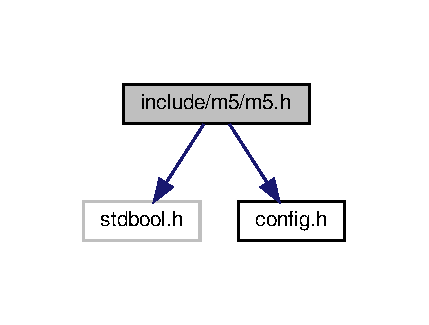
\includegraphics[width=206pt]{m5_8h__incl}
\end{center}
\end{figure}
This graph shows which files directly or indirectly include this file\+:
\nopagebreak
\begin{figure}[H]
\begin{center}
\leavevmode
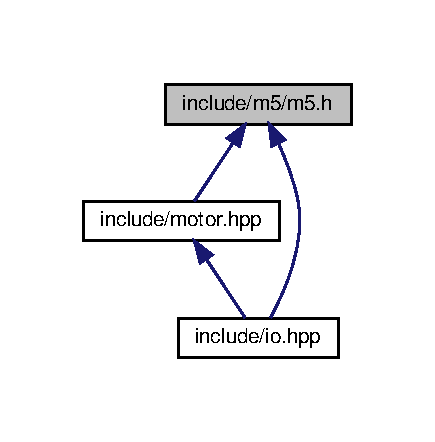
\includegraphics[width=221pt]{m5_8h__dep__incl}
\end{center}
\end{figure}
\subsection*{Functions}
\begin{DoxyCompactItemize}
\item 
int \hyperlink{m5_8h_a5b009d85753bf6e5052b9f51cf4c4b25}{m5\+\_\+power\+\_\+trans} ()
\begin{DoxyCompactList}\small\item\em Writes the next byte of the propulsion command packet to the M5s. \end{DoxyCompactList}\item 
void \hyperlink{m5_8h_a825b295706601422db8d5d0fa407e0bc}{m5\+\_\+power} (enum \hyperlink{config_8h_a2ee7466b8ebcae32e1e733f8067a6f9a}{thruster} t, float power)
\begin{DoxyCompactList}\small\item\em Sets thruster t to \char`\"{}power\char`\"{} power. \end{DoxyCompactList}\item 
void \hyperlink{m5_8h_aa580f305d0338c5fd86198bf4ac431a8}{m5\+\_\+power\+\_\+offer\+\_\+resume} ()
\begin{DoxyCompactList}\small\item\em Gives power to all the motors. \end{DoxyCompactList}\end{DoxyCompactItemize}


\subsection{Detailed Description}
Interface function definitions for Videoray M5 motors. 

\begin{DoxyAuthor}{Author}
Seth Girvan (Lord) 
\end{DoxyAuthor}


\subsection{Function Documentation}
\mbox{\Hypertarget{m5_8h_a825b295706601422db8d5d0fa407e0bc}\label{m5_8h_a825b295706601422db8d5d0fa407e0bc}} 
\index{m5.\+h@{m5.\+h}!m5\+\_\+power@{m5\+\_\+power}}
\index{m5\+\_\+power@{m5\+\_\+power}!m5.\+h@{m5.\+h}}
\subsubsection{\texorpdfstring{m5\+\_\+power()}{m5\_power()}}
{\footnotesize\ttfamily void m5\+\_\+power (\begin{DoxyParamCaption}\item[{enum \hyperlink{config_8h_a2ee7466b8ebcae32e1e733f8067a6f9a}{thruster}}]{t,  }\item[{float}]{power }\end{DoxyParamCaption})}



Sets thruster t to \char`\"{}power\char`\"{} power. 

The new value will not actually be transmitted until m5\+\_\+power\+\_\+offer\+\_\+resume is called.


\begin{DoxyParams}{Parameters}
{\em t} & The thruster that is being powered. \\
\hline
{\em power} & The amount of power, in range of \mbox{[}-\/1, 1\mbox{]}. \\
\hline
\end{DoxyParams}
\mbox{\Hypertarget{m5_8h_aa580f305d0338c5fd86198bf4ac431a8}\label{m5_8h_aa580f305d0338c5fd86198bf4ac431a8}} 
\index{m5.\+h@{m5.\+h}!m5\+\_\+power\+\_\+offer\+\_\+resume@{m5\+\_\+power\+\_\+offer\+\_\+resume}}
\index{m5\+\_\+power\+\_\+offer\+\_\+resume@{m5\+\_\+power\+\_\+offer\+\_\+resume}!m5.\+h@{m5.\+h}}
\subsubsection{\texorpdfstring{m5\+\_\+power\+\_\+offer\+\_\+resume()}{m5\_power\_offer\_resume()}}
{\footnotesize\ttfamily void m5\+\_\+power\+\_\+offer\+\_\+resume (\begin{DoxyParamCaption}{ }\end{DoxyParamCaption})}



Gives power to all the motors. 

Sets the most recent power value set for each thruster with m5\+\_\+power to be transmitted as soon as the next set of thrust values begin transmission.

Resumes transmission if it is currently paused. \mbox{\Hypertarget{m5_8h_a5b009d85753bf6e5052b9f51cf4c4b25}\label{m5_8h_a5b009d85753bf6e5052b9f51cf4c4b25}} 
\index{m5.\+h@{m5.\+h}!m5\+\_\+power\+\_\+trans@{m5\+\_\+power\+\_\+trans}}
\index{m5\+\_\+power\+\_\+trans@{m5\+\_\+power\+\_\+trans}!m5.\+h@{m5.\+h}}
\subsubsection{\texorpdfstring{m5\+\_\+power\+\_\+trans()}{m5\_power\_trans()}}
{\footnotesize\ttfamily int m5\+\_\+power\+\_\+trans (\begin{DoxyParamCaption}{ }\end{DoxyParamCaption})}



Writes the next byte of the propulsion command packet to the M5s. 

\begin{DoxyReturn}{Returns}
E\+OF on failure writing byte, 1 on packet completion, and zero on non-\/packet completion. 
\end{DoxyReturn}

\hypertarget{macrodef_8h}{}\section{include/macrodef.h File Reference}
\label{macrodef_8h}\index{include/macrodef.\+h@{include/macrodef.\+h}}


Helper macros for various parts of Nautical.  


\subsection*{Macros}
\begin{DoxyCompactItemize}
\item 
\mbox{\Hypertarget{macrodef_8h_ad0add60b29474b53705e3863a72935d4}\label{macrodef_8h_ad0add60b29474b53705e3863a72935d4}} 
\#define {\bfseries C\+O\+U\+N\+T\+OF}(a)~(sizeof(a)/sizeof(0\mbox{[}a\mbox{]})/((void $\ast$)a == (void $\ast$)\&a))
\item 
\mbox{\Hypertarget{macrodef_8h_a994e9792448fa94d193dc4c679a03ba6}\label{macrodef_8h_a994e9792448fa94d193dc4c679a03ba6}} 
\#define {\bfseries I\+N\+\_\+\+R\+A\+N\+GE}(min,  val,  max)~(min $<$= val \&\& val $<$= max)
\item 
\mbox{\Hypertarget{macrodef_8h_a0ed9e38823490c0ca01861f9506978d5}\label{macrodef_8h_a0ed9e38823490c0ca01861f9506978d5}} 
\#define {\bfseries T\+R\+U\+NC}(min,  val,  max)~(val $<$= min ? min \+: (val $>$= max ? max \+: val))
\item 
\mbox{\Hypertarget{macrodef_8h_a1df61a2ed0648e55628a10f9d662ad7b}\label{macrodef_8h_a1df61a2ed0648e55628a10f9d662ad7b}} 
\#define {\bfseries S\+T\+R\+I\+N\+G\+I\+F\+Y\+\_\+N}(a)~\#a
\item 
\mbox{\Hypertarget{macrodef_8h_a20b5fb7991df2f95c18b18f428032851}\label{macrodef_8h_a20b5fb7991df2f95c18b18f428032851}} 
\#define {\bfseries S\+T\+R\+I\+N\+G\+I\+F\+Y\+\_\+X}(a)~S\+T\+R\+I\+N\+G\+I\+F\+Y\+\_\+N(a)
\item 
\mbox{\Hypertarget{macrodef_8h_ac3aad8fca2e1594e51c7cf43fdbd674c}\label{macrodef_8h_ac3aad8fca2e1594e51c7cf43fdbd674c}} 
\#define {\bfseries C\+C\+\_\+\+N\+NN}(a,  b,  c)~a \#\# b \#\# c
\item 
\mbox{\Hypertarget{macrodef_8h_aaecffb50367b64f17cf53d6be33832c9}\label{macrodef_8h_aaecffb50367b64f17cf53d6be33832c9}} 
\#define {\bfseries C\+C\+\_\+\+X\+XX}(a,  b,  c)~C\+C\+\_\+\+N\+NN(a, b, c)
\item 
\mbox{\Hypertarget{macrodef_8h_aba1028403e85d5827afe41ecbf9c7f72}\label{macrodef_8h_aba1028403e85d5827afe41ecbf9c7f72}} 
\#define {\bfseries C\+C\+\_\+\+N\+XN}(a,  b,  c,  dum)~C\+C\+\_\+\+N\+NN(a \#\# dum, b, c \#\#dum)
\item 
\mbox{\Hypertarget{macrodef_8h_a8ca32837108d29eb4625f9312c254dc9}\label{macrodef_8h_a8ca32837108d29eb4625f9312c254dc9}} 
\#define {\bfseries S\+E\+T\+\_\+\+B\+I\+T\+\_\+\+H\+I\+GH}(reg,  bit)~reg $\vert$= (1\+U $<$$<$ bit)
\item 
\mbox{\Hypertarget{macrodef_8h_a342b6b1c94719d0d55e131114d690fad}\label{macrodef_8h_a342b6b1c94719d0d55e131114d690fad}} 
\#define {\bfseries S\+E\+T\+\_\+\+B\+I\+T\+\_\+\+L\+OW}(reg,  bit)~reg \&= $\sim$(1\+U $<$$<$ bit)
\item 
\mbox{\Hypertarget{macrodef_8h_a27d87ec86421947bafee84e2811ac5cd}\label{macrodef_8h_a27d87ec86421947bafee84e2811ac5cd}} 
\#define {\bfseries B\+I\+T\+\_\+\+V\+A\+L\+UE}(reg,  bit)~reg \& (1\+U $<$$<$ bit)
\item 
\mbox{\Hypertarget{macrodef_8h_ad2d787cd2c171fde13fcabf374389fe8}\label{macrodef_8h_ad2d787cd2c171fde13fcabf374389fe8}} 
\#define {\bfseries T\+O\+G\+G\+L\+E\+\_\+\+B\+IT}(reg,  bit)~reg $^\wedge$= (1\+U $<$$<$ bit)
\end{DoxyCompactItemize}


\subsection{Detailed Description}
Helper macros for various parts of Nautical. 

\begin{DoxyAuthor}{Author}
Seth Girvan (Lord) 
\end{DoxyAuthor}

\hypertarget{matrix_8h}{}\section{include/matrix.h File Reference}
\label{matrix_8h}\index{include/matrix.\+h@{include/matrix.\+h}}


Function declarations for matrix operations.  


{\ttfamily \#include $<$Arduino.\+h$>$}\newline
Include dependency graph for matrix.\+h\+:\nopagebreak
\begin{figure}[H]
\begin{center}
\leavevmode
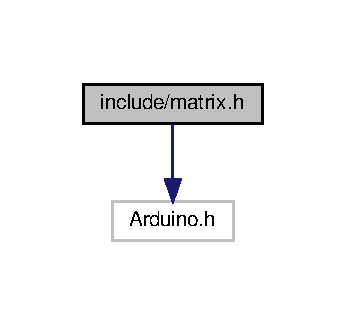
\includegraphics[width=166pt]{matrix_8h__incl}
\end{center}
\end{figure}
\subsection*{Functions}
\begin{DoxyCompactItemize}
\item 
void \hyperlink{matrix_8h_a806a9984da7f155de1d72e4409fe41a5}{print} (float $\ast$A, int m, int n)
\begin{DoxyCompactList}\small\item\em Print real matrix to terminal. \end{DoxyCompactList}\item 
void \hyperlink{matrix_8h_ad2ee4eac600dbdf6950781957e8f7d14}{copy} (float $\ast$A, int n, int m, float $\ast$B)
\begin{DoxyCompactList}\small\item\em Copies the elements from one matrix to another. \end{DoxyCompactList}\item 
void \hyperlink{matrix_8h_a50d178d74f498878c116b677804f8a9d}{multiply} (float $\ast$A, float $\ast$B, int m, int p, int n, float $\ast$C)
\begin{DoxyCompactList}\small\item\em Multiplies two matrices together. \end{DoxyCompactList}\item 
void \hyperlink{matrix_8h_af4b108d76582e8d66b1c19dd1878bcbe}{add} (float $\ast$A, float $\ast$B, int m, int n, float $\ast$C)
\begin{DoxyCompactList}\small\item\em Adds two matrices together. \end{DoxyCompactList}\item 
void \hyperlink{matrix_8h_a4a1032bae9b5fdfaaaef2ea17ab21ef3}{subtract} (float $\ast$A, float $\ast$B, int m, int n, float $\ast$C)
\begin{DoxyCompactList}\small\item\em Subtracts two matrices. \end{DoxyCompactList}\item 
void \hyperlink{matrix_8h_a437752bd1f9b3c62c2844ed921e17b70}{transpose} (float $\ast$A, int m, int n, float $\ast$C)
\begin{DoxyCompactList}\small\item\em Takes the transpose of a matrix. \end{DoxyCompactList}\item 
void \hyperlink{matrix_8h_ae6482d1e4de05e954edf47b04492873a}{scale} (float $\ast$A, int m, int n, float k)
\begin{DoxyCompactList}\small\item\em Multiplies a matrix by a scalar. \end{DoxyCompactList}\item 
int \hyperlink{matrix_8h_af73a219fb4514bdf2337b8b8b7600b0a}{invert} (float $\ast$A, int n)
\begin{DoxyCompactList}\small\item\em Takes the inverse of a matrix. \end{DoxyCompactList}\end{DoxyCompactItemize}


\subsection{Detailed Description}
Function declarations for matrix operations. 

Matrices are stored in 1-\/D arrays. To access a cell, use \mbox{[}r$\ast$n+c\mbox{]} instead of \mbox{[}r\mbox{]}\mbox{[}c\mbox{]}.

\begin{DoxyAuthor}{Author}
David Zhang (Davarco) 
\end{DoxyAuthor}


\subsection{Function Documentation}
\mbox{\Hypertarget{matrix_8h_af4b108d76582e8d66b1c19dd1878bcbe}\label{matrix_8h_af4b108d76582e8d66b1c19dd1878bcbe}} 
\index{matrix.\+h@{matrix.\+h}!add@{add}}
\index{add@{add}!matrix.\+h@{matrix.\+h}}
\subsubsection{\texorpdfstring{add()}{add()}}
{\footnotesize\ttfamily void add (\begin{DoxyParamCaption}\item[{float $\ast$}]{A,  }\item[{float $\ast$}]{B,  }\item[{int}]{m,  }\item[{int}]{n,  }\item[{float $\ast$}]{C }\end{DoxyParamCaption})}



Adds two matrices together. 


\begin{DoxyParams}{Parameters}
{\em A} & The first matrix. \\
\hline
{\em B} & The second matrix. \\
\hline
{\em m} & The number of rows in A and B. \\
\hline
{\em n} & The number of columns in A and B. \\
\hline
{\em C} & The added matrix. \\
\hline
\end{DoxyParams}
\mbox{\Hypertarget{matrix_8h_ad2ee4eac600dbdf6950781957e8f7d14}\label{matrix_8h_ad2ee4eac600dbdf6950781957e8f7d14}} 
\index{matrix.\+h@{matrix.\+h}!copy@{copy}}
\index{copy@{copy}!matrix.\+h@{matrix.\+h}}
\subsubsection{\texorpdfstring{copy()}{copy()}}
{\footnotesize\ttfamily void copy (\begin{DoxyParamCaption}\item[{float $\ast$}]{A,  }\item[{int}]{n,  }\item[{int}]{m,  }\item[{float $\ast$}]{B }\end{DoxyParamCaption})}



Copies the elements from one matrix to another. 


\begin{DoxyParams}{Parameters}
{\em A} & The matrix from where elements are copied from. \\
\hline
{\em m} & The number of rows in A and B. \\
\hline
{\em n} & The number of columns in A and B. \\
\hline
{\em B} & The matrix where elements are written to. \\
\hline
\end{DoxyParams}
\mbox{\Hypertarget{matrix_8h_af73a219fb4514bdf2337b8b8b7600b0a}\label{matrix_8h_af73a219fb4514bdf2337b8b8b7600b0a}} 
\index{matrix.\+h@{matrix.\+h}!invert@{invert}}
\index{invert@{invert}!matrix.\+h@{matrix.\+h}}
\subsubsection{\texorpdfstring{invert()}{invert()}}
{\footnotesize\ttfamily int invert (\begin{DoxyParamCaption}\item[{float $\ast$}]{A,  }\item[{int}]{n }\end{DoxyParamCaption})}



Takes the inverse of a matrix. 


\begin{DoxyParams}{Parameters}
{\em A} & The input matrix, must be square. \\
\hline
{\em n} & The number of rows and columns in A. \\
\hline
{\em B} & The inverted matrix. \\
\hline
\end{DoxyParams}
\mbox{\Hypertarget{matrix_8h_a50d178d74f498878c116b677804f8a9d}\label{matrix_8h_a50d178d74f498878c116b677804f8a9d}} 
\index{matrix.\+h@{matrix.\+h}!multiply@{multiply}}
\index{multiply@{multiply}!matrix.\+h@{matrix.\+h}}
\subsubsection{\texorpdfstring{multiply()}{multiply()}}
{\footnotesize\ttfamily void multiply (\begin{DoxyParamCaption}\item[{float $\ast$}]{A,  }\item[{float $\ast$}]{B,  }\item[{int}]{m,  }\item[{int}]{p,  }\item[{int}]{n,  }\item[{float $\ast$}]{C }\end{DoxyParamCaption})}



Multiplies two matrices together. 


\begin{DoxyParams}{Parameters}
{\em A} & The first matrix. \\
\hline
{\em B} & The second matrix. \\
\hline
{\em m} & The number of rows in A. \\
\hline
{\em p} & The number of columns in A and number of rows in B. \\
\hline
{\em n} & The number of columns in B. \\
\hline
{\em C} & The multiplied matrix of order mxn. \\
\hline
\end{DoxyParams}
\mbox{\Hypertarget{matrix_8h_a806a9984da7f155de1d72e4409fe41a5}\label{matrix_8h_a806a9984da7f155de1d72e4409fe41a5}} 
\index{matrix.\+h@{matrix.\+h}!print@{print}}
\index{print@{print}!matrix.\+h@{matrix.\+h}}
\subsubsection{\texorpdfstring{print()}{print()}}
{\footnotesize\ttfamily void print (\begin{DoxyParamCaption}\item[{float $\ast$}]{A,  }\item[{int}]{m,  }\item[{int}]{n }\end{DoxyParamCaption})}



Print real matrix to terminal. 


\begin{DoxyParams}{Parameters}
{\em A} & The matrix that is printed. \\
\hline
{\em m} & The number of rows in A. \\
\hline
{\em n} & The number of columns in B. \\
\hline
{\em msg} & The header message preceding the matrix. \\
\hline
\end{DoxyParams}
\mbox{\Hypertarget{matrix_8h_ae6482d1e4de05e954edf47b04492873a}\label{matrix_8h_ae6482d1e4de05e954edf47b04492873a}} 
\index{matrix.\+h@{matrix.\+h}!scale@{scale}}
\index{scale@{scale}!matrix.\+h@{matrix.\+h}}
\subsubsection{\texorpdfstring{scale()}{scale()}}
{\footnotesize\ttfamily void scale (\begin{DoxyParamCaption}\item[{float $\ast$}]{A,  }\item[{int}]{m,  }\item[{int}]{n,  }\item[{float}]{k }\end{DoxyParamCaption})}



Multiplies a matrix by a scalar. 


\begin{DoxyParams}{Parameters}
{\em A} & The input matrix, where the results are written to as well. \\
\hline
{\em m} & The number of rows in A. \\
\hline
{\em n} & The number of columns in A. \\
\hline
{\em k} & The scalar value. \\
\hline
\end{DoxyParams}
\mbox{\Hypertarget{matrix_8h_a4a1032bae9b5fdfaaaef2ea17ab21ef3}\label{matrix_8h_a4a1032bae9b5fdfaaaef2ea17ab21ef3}} 
\index{matrix.\+h@{matrix.\+h}!subtract@{subtract}}
\index{subtract@{subtract}!matrix.\+h@{matrix.\+h}}
\subsubsection{\texorpdfstring{subtract()}{subtract()}}
{\footnotesize\ttfamily void subtract (\begin{DoxyParamCaption}\item[{float $\ast$}]{A,  }\item[{float $\ast$}]{B,  }\item[{int}]{m,  }\item[{int}]{n,  }\item[{float $\ast$}]{C }\end{DoxyParamCaption})}



Subtracts two matrices. 


\begin{DoxyParams}{Parameters}
{\em A} & The first matrix. \\
\hline
{\em B} & The second matrix. \\
\hline
{\em m} & The number of rows in A and B. \\
\hline
{\em n} & The number of columns in A and B. \\
\hline
{\em C} & The subtracted matrix. \\
\hline
\end{DoxyParams}
\mbox{\Hypertarget{matrix_8h_a437752bd1f9b3c62c2844ed921e17b70}\label{matrix_8h_a437752bd1f9b3c62c2844ed921e17b70}} 
\index{matrix.\+h@{matrix.\+h}!transpose@{transpose}}
\index{transpose@{transpose}!matrix.\+h@{matrix.\+h}}
\subsubsection{\texorpdfstring{transpose()}{transpose()}}
{\footnotesize\ttfamily void transpose (\begin{DoxyParamCaption}\item[{float $\ast$}]{A,  }\item[{int}]{m,  }\item[{int}]{n,  }\item[{float $\ast$}]{C }\end{DoxyParamCaption})}



Takes the transpose of a matrix. 


\begin{DoxyParams}{Parameters}
{\em A} & The input matrix to transpose. \\
\hline
{\em m} & The number of rows in A. \\
\hline
{\em n} & The number of columns in A. \\
\hline
{\em B} & The transposed matrix of order nxm. \\
\hline
\end{DoxyParams}

\hypertarget{motor_8hpp}{}\section{include/motor.hpp File Reference}
\label{motor_8hpp}\index{include/motor.\+hpp@{include/motor.\+hpp}}


Helper class to use all of the motors at once and do computations.  


{\ttfamily \#include \char`\"{}m5/m5.\+h\char`\"{}}\newline
{\ttfamily \#include \char`\"{}config.\+h\char`\"{}}\newline
{\ttfamily \#include \char`\"{}pid.\+hpp\char`\"{}}\newline
Include dependency graph for motor.\+hpp\+:
\nopagebreak
\begin{figure}[H]
\begin{center}
\leavevmode
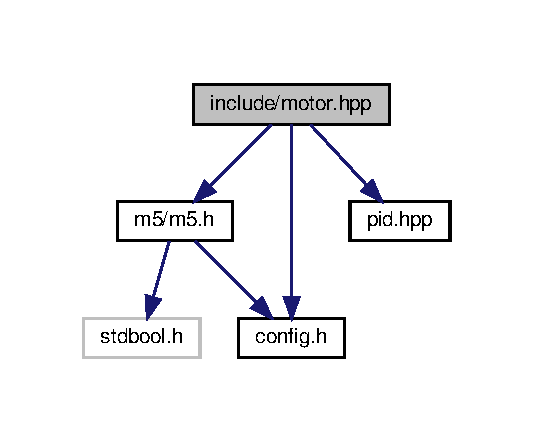
\includegraphics[width=256pt]{motor_8hpp__incl}
\end{center}
\end{figure}
This graph shows which files directly or indirectly include this file\+:
\nopagebreak
\begin{figure}[H]
\begin{center}
\leavevmode
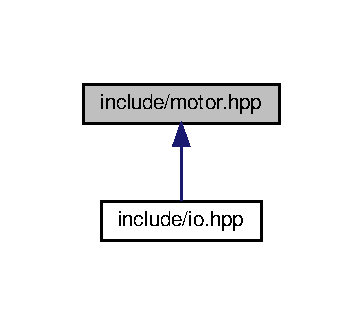
\includegraphics[width=174pt]{motor_8hpp__dep__incl}
\end{center}
\end{figure}
\subsection*{Data Structures}
\begin{DoxyCompactItemize}
\item 
struct \hyperlink{structMotors}{Motors}
\begin{DoxyCompactList}\small\item\em Helper class for motors. \end{DoxyCompactList}\end{DoxyCompactItemize}
\subsection*{Macros}
\begin{DoxyCompactItemize}
\item 
\#define \hyperlink{motor_8hpp_ae0edb34f25808edbd9c240ce645d36db}{P\+A\+U\+S\+E\+\_\+\+T\+I\+ME}~4500
\end{DoxyCompactItemize}


\subsection{Detailed Description}
Helper class to use all of the motors at once and do computations. 

\begin{DoxyAuthor}{Author}
David Zhang 
\end{DoxyAuthor}


\subsection{Macro Definition Documentation}
\mbox{\Hypertarget{motor_8hpp_ae0edb34f25808edbd9c240ce645d36db}\label{motor_8hpp_ae0edb34f25808edbd9c240ce645d36db}} 
\index{motor.\+hpp@{motor.\+hpp}!P\+A\+U\+S\+E\+\_\+\+T\+I\+ME@{P\+A\+U\+S\+E\+\_\+\+T\+I\+ME}}
\index{P\+A\+U\+S\+E\+\_\+\+T\+I\+ME@{P\+A\+U\+S\+E\+\_\+\+T\+I\+ME}!motor.\+hpp@{motor.\+hpp}}
\subsubsection{\texorpdfstring{P\+A\+U\+S\+E\+\_\+\+T\+I\+ME}{PAUSE\_TIME}}
{\footnotesize\ttfamily \#define P\+A\+U\+S\+E\+\_\+\+T\+I\+ME~4500}

Startup time for motors after sub is unkilled. 
\hypertarget{pid_8hpp}{}\section{include/pid.hpp File Reference}
\label{pid_8hpp}\index{include/pid.\+hpp@{include/pid.\+hpp}}


Helper class to compute \hyperlink{structPID}{P\+ID} for motors.  


This graph shows which files directly or indirectly include this file\+:
\nopagebreak
\begin{figure}[H]
\begin{center}
\leavevmode
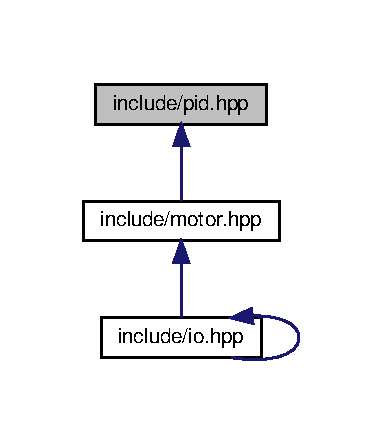
\includegraphics[width=174pt]{pid_8hpp__dep__incl}
\end{center}
\end{figure}
\subsection*{Data Structures}
\begin{DoxyCompactItemize}
\item 
struct \hyperlink{structPID}{P\+ID}
\end{DoxyCompactItemize}


\subsection{Detailed Description}
Helper class to compute \hyperlink{structPID}{P\+ID} for motors. 

\begin{DoxyAuthor}{Author}
David Zhang 
\end{DoxyAuthor}

%--- End generated contents ---

% Index
\backmatter
\newpage
\phantomsection
\clearemptydoublepage
\addcontentsline{toc}{chapter}{Index}
\printindex

\end{document}
